\documentclass[10pt]{beamer}

% --- PAQUETES REQUERIDOS ---
\usepackage[utf8]{inputenc}
\usepackage[T1]{fontenc}
\usepackage[spanish,es-nodecimaldot]{babel}
\usepackage{amsmath,amsfonts,amssymb}
\usepackage{graphicx}
\usepackage{booktabs}
\usepackage{array}
\usepackage{xcolor}
\usepackage{tikz}
\usepackage{ragged2e}

% --- CONFIGURACIÓN DE RUTAS DE IMÁGENES ---
\graphicspath{{./}{../../}{../}}

% --- PALETA DE COLORES INSTITUCIONAL UAGRM ---
\definecolor{dodgerblue}{RGB}{30, 144, 255}
\definecolor{darkblue}{RGB}{0, 51, 102}
\definecolor{firebrick}{RGB}{178, 34, 34}
\definecolor{lightblue}{RGB}{232, 244, 250}
\definecolor{boxborder}{RGB}{0, 102, 153}
\definecolor{softgray}{RGB}{248, 249, 250}
\definecolor{darkgreen}{RGB}{34, 139, 34}
\definecolor{softgreen}{RGB}{232, 245, 233}
\definecolor{softred}{RGB}{255, 235, 238}
\definecolor{amber}{RGB}{245, 124, 0}

% --- CONFIGURACIÓN DEL TEMA BEAMER ---
\usetheme{Madrid}
\usecolortheme{default}

\setbeamercolor{palette primary}{bg=dodgerblue, fg=white}
\setbeamercolor{palette secondary}{bg=darkblue, fg=white}
\setbeamercolor{palette tertiary}{bg=dodgerblue, fg=white}
\setbeamercolor{frametitle}{bg=darkblue, fg=white}
\setbeamercolor{title}{fg=darkblue}
\setbeamercolor{subtitle}{fg=dodgerblue}
\setbeamercolor{block title}{bg=darkblue, fg=white}
\setbeamercolor{block body}{bg=lightblue, fg=black}
\setbeamercolor{block title alerted}{bg=firebrick, fg=white}
\setbeamercolor{block body alerted}{bg=softred, fg=black}
\setbeamercolor{block title example}{bg=darkgreen, fg=white}
\setbeamercolor{block body example}{bg=softgreen, fg=black}

\setbeamertemplate{navigation symbols}{}

% --- VIÑETAS PERSONALIZADAS ---
\setbeamertemplate{itemize item}{\color{dodgerblue}\scriptsize$\blacksquare$}
\setbeamertemplate{itemize subitem}{\color{darkblue}\tiny$\blacktriangleright$}

% --- PIE DE PÁGINA TRICOLOR INSTITUCIONAL ---
\setbeamertemplate{footline}{
  \leavevmode%
  \hbox{%
  \begin{beamercolorbox}[wd=.35\paperwidth,ht=2.5ex,dp=1ex,center]{palette secondary}%
    \footnotesize MSc. Anselmo Salguero Arano
  \end{beamercolorbox}%
  \begin{beamercolorbox}[wd=.45\paperwidth,ht=2.5ex,dp=1ex,center]{palette primary}%
    \footnotesize MAT 260 | Reporte Ejecutivo \& Diagnóstico
  \end{beamercolorbox}%
  \begin{beamercolorbox}[wd=.20\paperwidth,ht=2.5ex,dp=1ex,right]{palette secondary}%
    \footnotesize \textbf{\insertframenumber{} / \inserttotalframenumber}\hspace*{2ex}
  \end{beamercolorbox}}%
  \vskip0pt%
}

% --- COMANDOS PERSONALIZADOS DE CAJAS ---
\newcommand{\formulabox}[1]{%
  \begin{center}
  \begin{tikzpicture}
    \node[fill=lightblue, draw=boxborder, line width=1pt, rounded corners=4pt, inner sep=4pt, text width=0.92\textwidth, align=left] {#1};
  \end{tikzpicture}
  \end{center}
}

\newcommand{\alertbox}[1]{%
  \begin{center}
  \begin{tikzpicture}
    \node[fill=softred, draw=firebrick, line width=1pt, rounded corners=4pt, inner sep=4pt, text width=0.92\textwidth, align=left] {#1};
  \end{tikzpicture}
  \end{center}
}

\newcommand{\greenbox}[1]{%
  \begin{center}
  \begin{tikzpicture}
    \node[fill=softgreen, draw=darkgreen, line width=1pt, rounded corners=4pt, inner sep=4pt, text width=0.92\textwidth, align=left] {#1};
  \end{tikzpicture}
  \end{center}
}

% --- METADATOS DE LA PRESENTACIÓN ---
\title[Informe Ejecutivo \& Diagnóstico]{REPORTE EJECUTIVO DE AVANCE EN AULA VIRTUAL Y ANÁLISIS ESTADÍSTICO DIAGNÓSTICO}
\subtitle{Asignatura: Estadística II (MAT 260 - Grupo EP) | Semestre II-2026}
\author[MSc. Anselmo Salguero A.]{MSc. Ing. Anselmo Salguero Arano}
\institute[UAGRM]{Universidad Autónoma Gabriel René Moreno\\Facultad de Ciencias Contables, Auditoría, Sistemas de Control de Gestión y Finanzas}
\date{01 de Septiembre de 2026}

\begin{document}

% =========================================================================
% PORTADA
% =========================================================================
\begin{frame}[plain]
  \centering
  \vspace*{-0.2cm}
  \begin{minipage}{0.30\textwidth}
    \centering
    
\includegraphics[width=0.65\linewidth]{Logouagrm.png}
  \end{minipage}
  \hfill
  \begin{minipage}{0.30\textwidth}
    \centering
    
\includegraphics[width=0.65\linewidth]{Logocont.png}
  \end{minipage}
  
  \vspace{0.25cm}
  {\fontsize{11}{13}\selectfont \textbf{\color{darkblue}UNIVERSIDAD AUTÓNOMA GABRIEL RENÉ MORENO}}\\[0.05cm]
  {\fontsize{8}{10}\selectfont \color{darkblue}Facultad de Ciencias Contables, Auditoría, Sistemas de Control de Gestión y Finanzas}\\[0.05cm]
  {\fontsize{8}{10}\selectfont \color{dodgerblue}\textbf{Carrera de Contaduría Pública — Estadística II (MAT 260)}}\\[0.25cm]
  
  \begin{beamercolorbox}[sep=4pt,center,rounded=true,shadow=true]{palette primary}
    {\fontsize{10}{12}\selectfont \textbf{INFORME EJECUTIVO DE PARTICIPACIÓN MOODLE Y ANÁLISIS ESTADÍSTICO DE LA ENCUESTA INICIAL}}
  \end{beamercolorbox}
  
  \vspace{0.25cm}
  {\fontsize{8.5}{11}\selectfont \textbf{Docente Titular:} MSc. Ing. Anselmo Salguero Arano}\\[0.05cm]
  {\fontsize{7.5}{9.5}\selectfont \textbf{Semestre Académico:} II-2026 \quad | \quad \textbf{Fecha de Corte:} 01 de Septiembre de 2026}
\end{frame}

% =========================================================================
% AGENDA / CONTENIDO
% =========================================================================
\begin{frame}{Estructura del Informe Ejecutivo}
  \tableofcontents
\end{frame}

% =========================================================================
% SECCIÓN 1: SEGUIMIENTO EN MOODLE
% =========================================================================
\section{Módulo I: Auditoría y Seguimiento en Aula Virtual Moodle ($N=44$)}

\begin{frame}{1.1 Cuadro de Mando y KPIs Globales de Inicio}
  \begin{columns}[T]
    \begin{column}{0.50\textwidth}
      \begin{block}{Indicadores de Participación ($N=44$)}
        \fontsize{7.5}{9.5}\selectfont
        \begin{tabular}{lcc}
          \toprule
          \textbf{Métrica Clave} & \textbf{Est.} & \textbf{\% Rel.} \\
          \midrule
          Matriculados Oficiales & \textbf{44} & 100.0\% \\
          Acceso Efectivo ($\ge 1$ act.) & \textbf{40} & \textbf{90.9\%} \\
          \alert{Sin Acceso (0 act.)} & \alert{\textbf{4}} & \alert{\textbf{9.1\%}} \\
          \midrule
          Grupo WhatsApp Oficial & 39 & 88.6\% \\
          Lecciones Teóricas 1 a 4 & 30 & 68.2\% \\
          Examen Diagnóstico (40 P.) & 25 & 56.8\% \\
          Memoria de Cálculo PDF & 22 & 50.0\% \\
          Encuesta Google Forms & 19 & 43.2\% \\
          \bottomrule
        \end{tabular}
      \end{block}
    \end{column}
    
    \begin{column}{0.48\textwidth}
      \greenbox{
        \textbf{Diagnóstico Operativo Inicial:}\\[0.1cm]
        \fontsize{7.5}{9.5}\selectfont
        $\blacktriangleright$ \textbf{Cobertura Exitosa:} El $90.9\%$ de los matriculados ingresó e interactuó en la primera semana.\\
        $\blacktriangleright$ \textbf{Comunicación Fluida:} $88.6\%$ integrado en el grupo oficial de WhatsApp.\\
        $\blacktriangleright$ \textbf{Alerta Inmediata:} 4 estudiantes requieren intervención directa por no registrar ingresos.
      }
    \end{column}
  \end{columns}
\end{frame}

\begin{frame}{1.2 Segmentación del Alumnado por Nivel de Actividad}
  \begin{columns}[c]
    \begin{column}{0.52\textwidth}
      \centering
      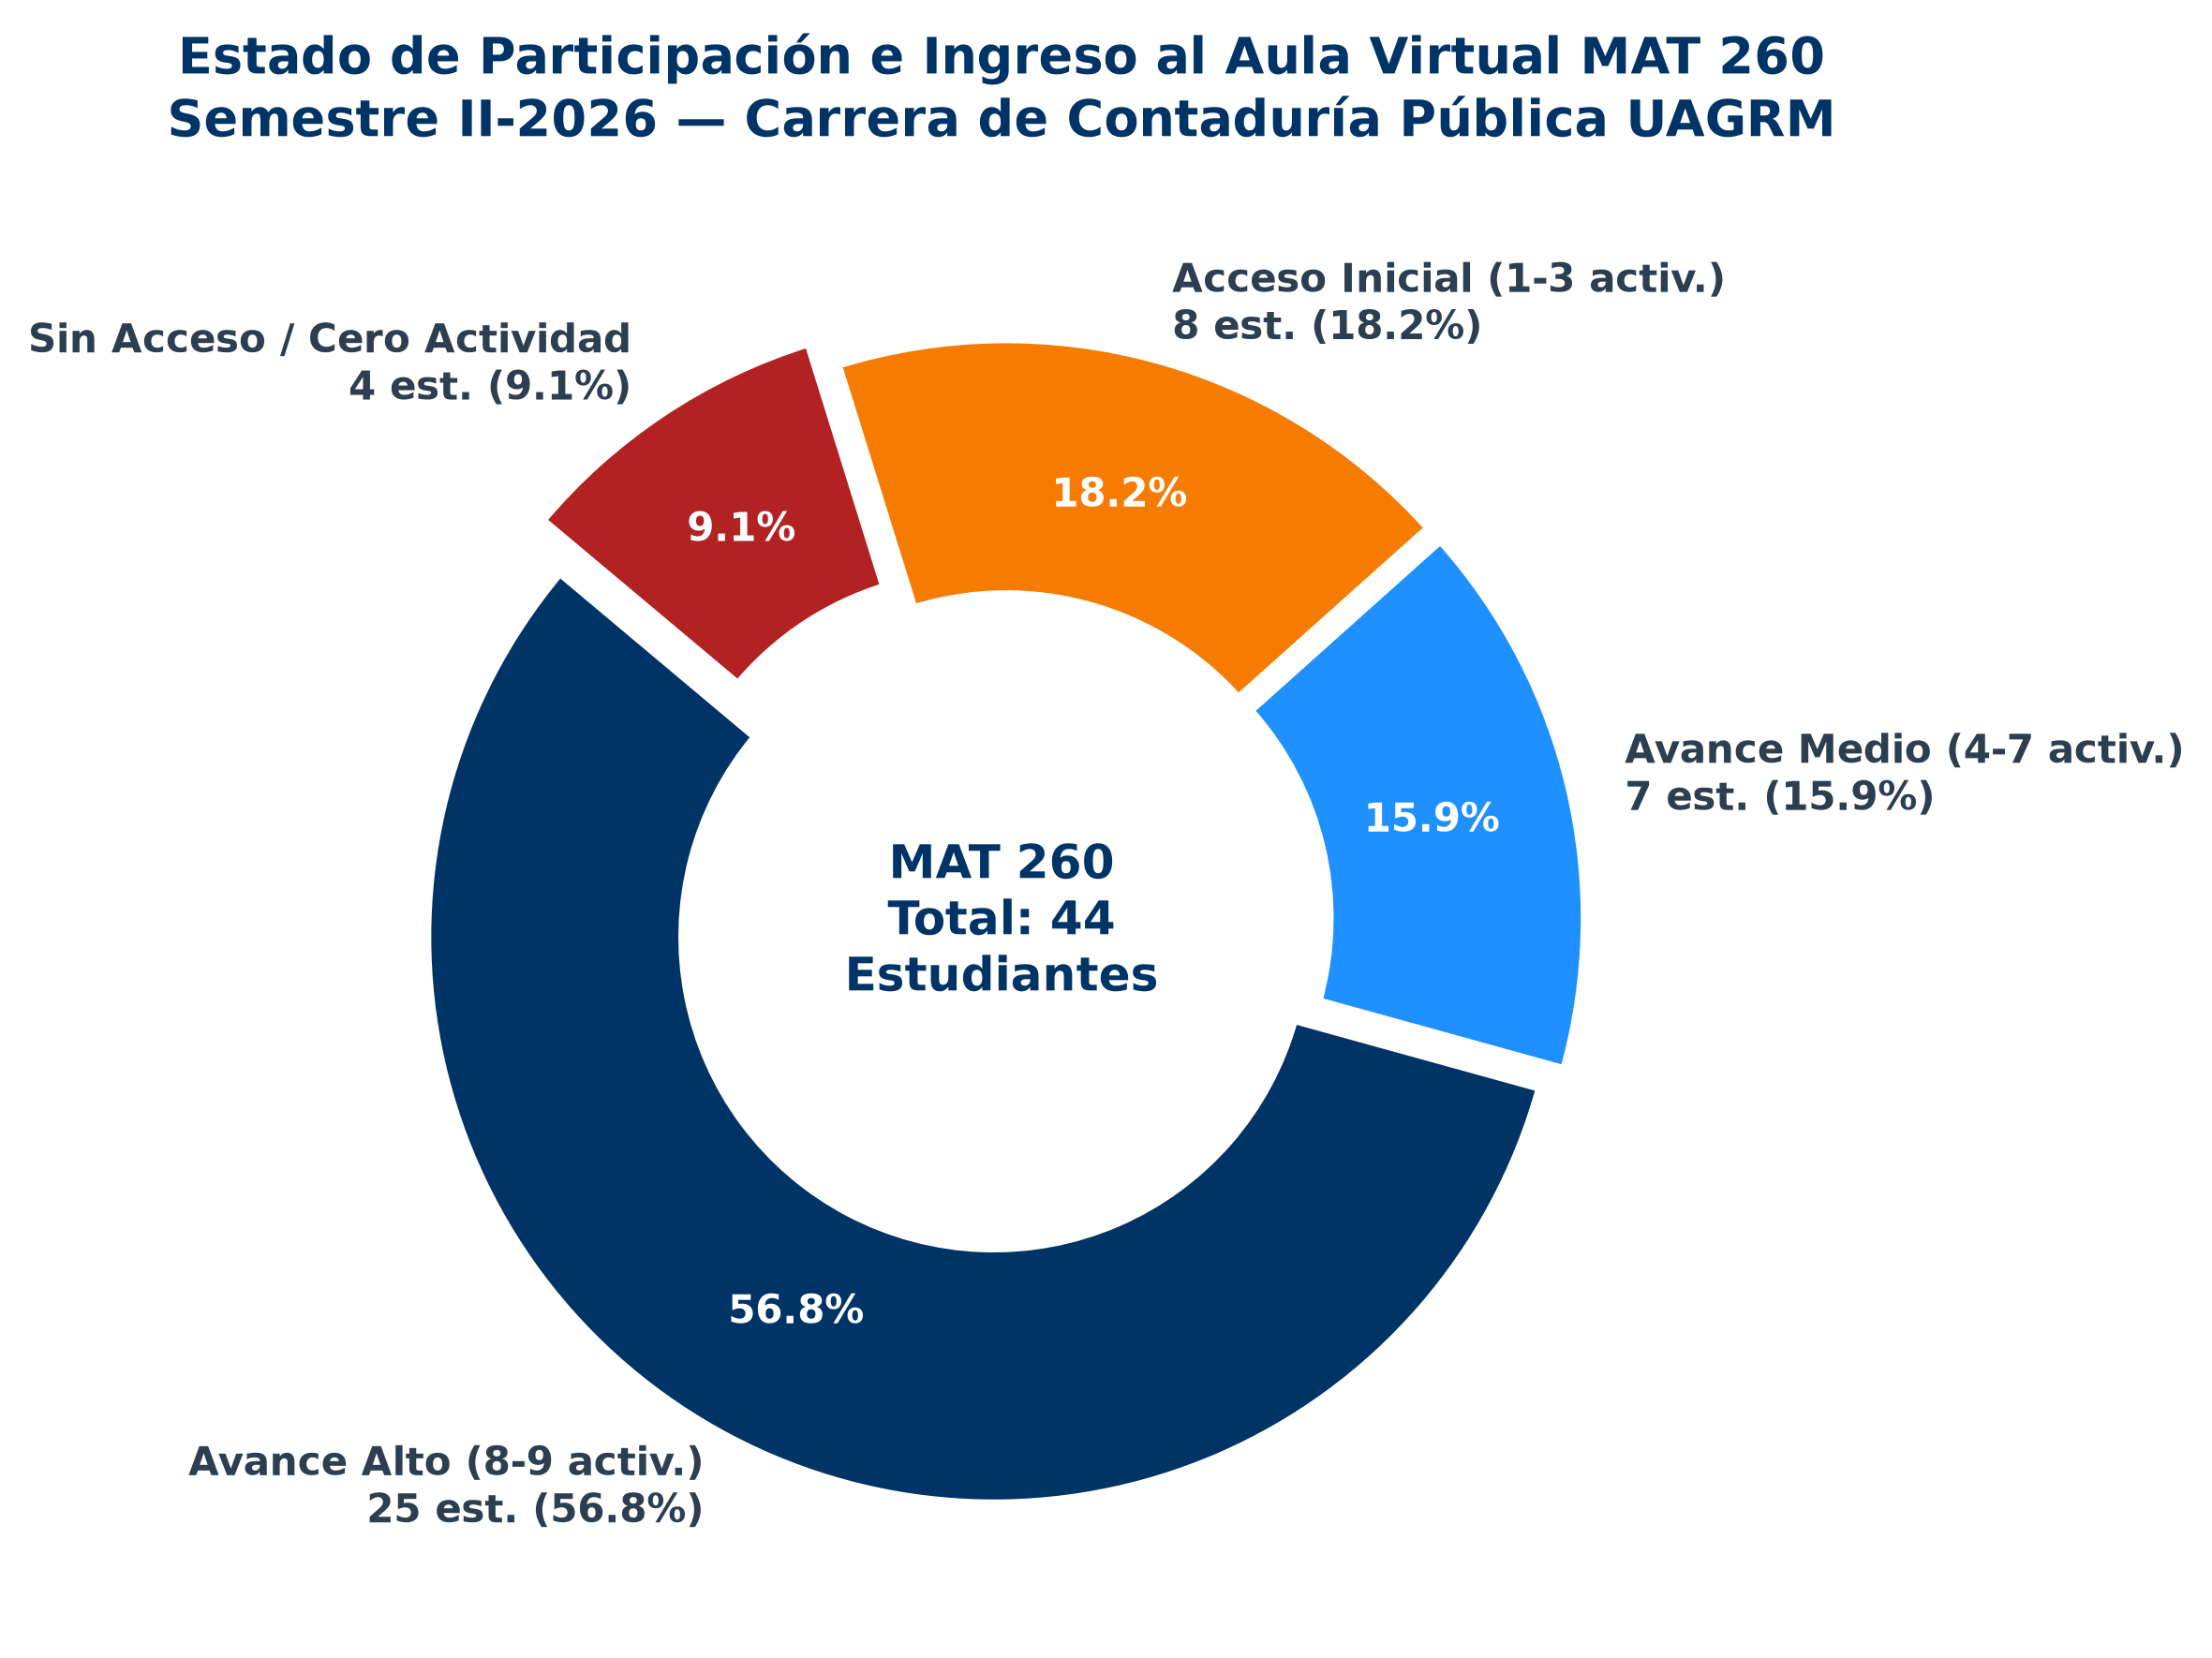
\includegraphics[width=\linewidth]{01_grafico_participacion_global_torta.png}
    \end{column}
    \begin{column}{0.46\textwidth}
      \begin{block}{Distribución por Categorías}
        \fontsize{7.5}{9.5}\selectfont
        \begin{itemize}
          \item \textbf{Avance Alto (8-9 act.):} 25 est. ($56.8\%$). Han cubierto lecciones, diagnóstico y memoria.
          \item \textbf{Avance Medio (4-7 act.):} 7 est. ($15.9\%$). Lectura de lecciones en desarrollo.
          \item \textbf{Acceso Inicial (1-3 act.):} 8 est. ($18.2\%$). Solo avisos y programa analítico.
          \item \alert{\textbf{Sin Acceso (0 act.):}} 4 est. ($9.1\%$). Sin conexión registrada.
        \end{itemize}
      \end{block}
    \end{column}
  \end{columns}
\end{frame}

\begin{frame}{1.3 Alerta Prioritaria: Estudiantes Sin Acceso a Plataforma}
  \alertbox{
    \textbf{Acción Docente Urgente:} Los siguientes 4 estudiantes no registran actividad en Moodle:
  }
  \vspace{0.15cm}
  
  \centering
  \fontsize{7.5}{9.5}\selectfont
  \begin{tabular}{clllc}
    \toprule
    \textbf{N°} & \textbf{Estudiante} & \textbf{Correo Electrónico} & \textbf{Teléfono} & \textbf{Acción} \\
    \midrule
    1 & CESPEDES DELGADILLO BRAYAN R. & \texttt{briantcespedes884@gmail.com} & *No reg.* & Aula Presencial \\
    2 & TAPIA PADILLA ANYELY & \texttt{anyelytapia120@gmail.com} & *No reg.* & Aula Presencial \\
    3 & \textbf{VEJAR CHAMBI ESMERALDA} & \texttt{luciachambiflores9@gmail.com} & \textbf{77085475} & \textbf{WhatsApp Directo} \\
    4 & ZEPITA ALEJANDRA KATHERINNE & \texttt{az324236@gmail.com} & *No reg.* & Aula Presencial \\
    \bottomrule
  \end{tabular}
  
  \vspace{0.25cm}
  \formulabox{
    \fontsize{7.5}{9.5}\selectfont
    \textbf{Estrategia de Rescate:} En el caso de \textbf{Esmeralda Vejar} se cuenta con número móvil directo para llamada. En los otros 3 casos, verificar asistencia en la lista física de clase.
  }
\end{frame}

\begin{frame}{1.4 Tasa de Avance por Lección y Actividad en Moodle}
  \centering
  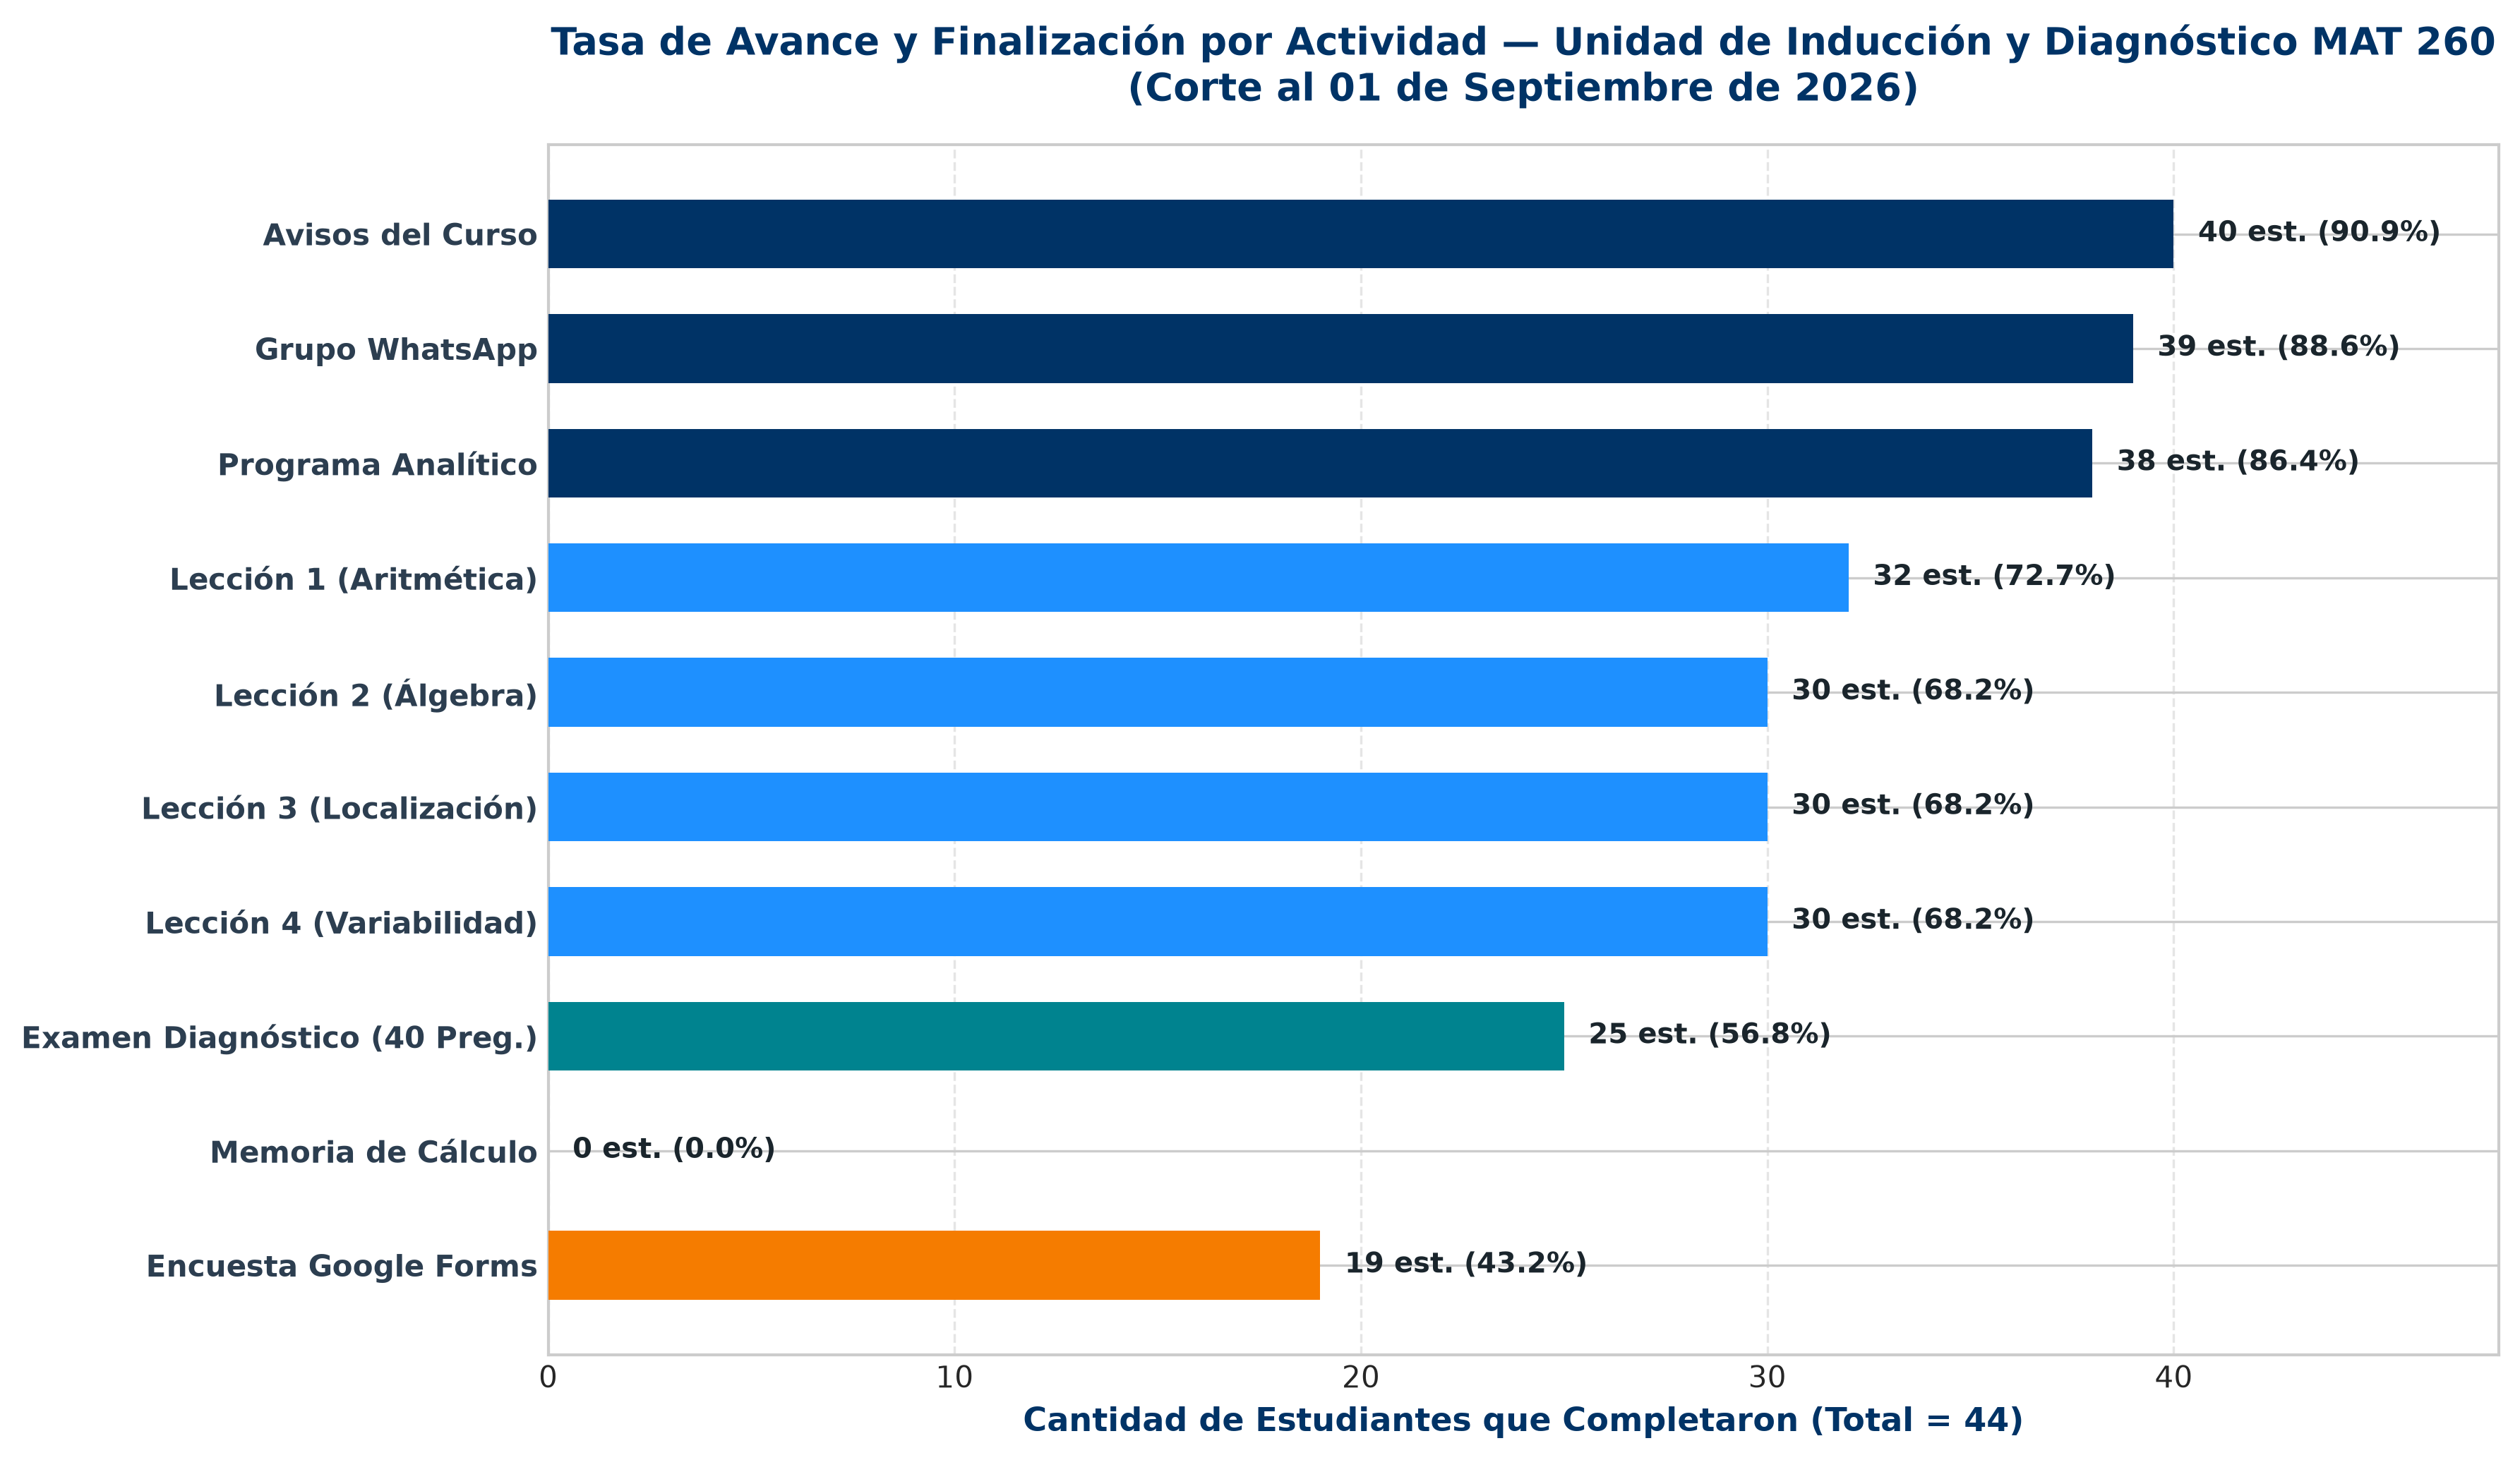
\includegraphics[width=0.92\linewidth]{03_grafico_embudo_actividades_barras.png}
  
  \vspace{0.1cm}
  \fontsize{7.5}{9.5}\selectfont
  \textbf{Observación:} La tasa de completitud se mantiene por encima del $68\%$ en las 4 lecciones de inducción (Aritmética, Álgebra, Localización y Variabilidad).
\end{frame}

\begin{frame}{1.5 Estado de la Encuesta Inicial en Google Forms}
  \begin{columns}[c]
    \begin{column}{0.54\textwidth}
      \centering
      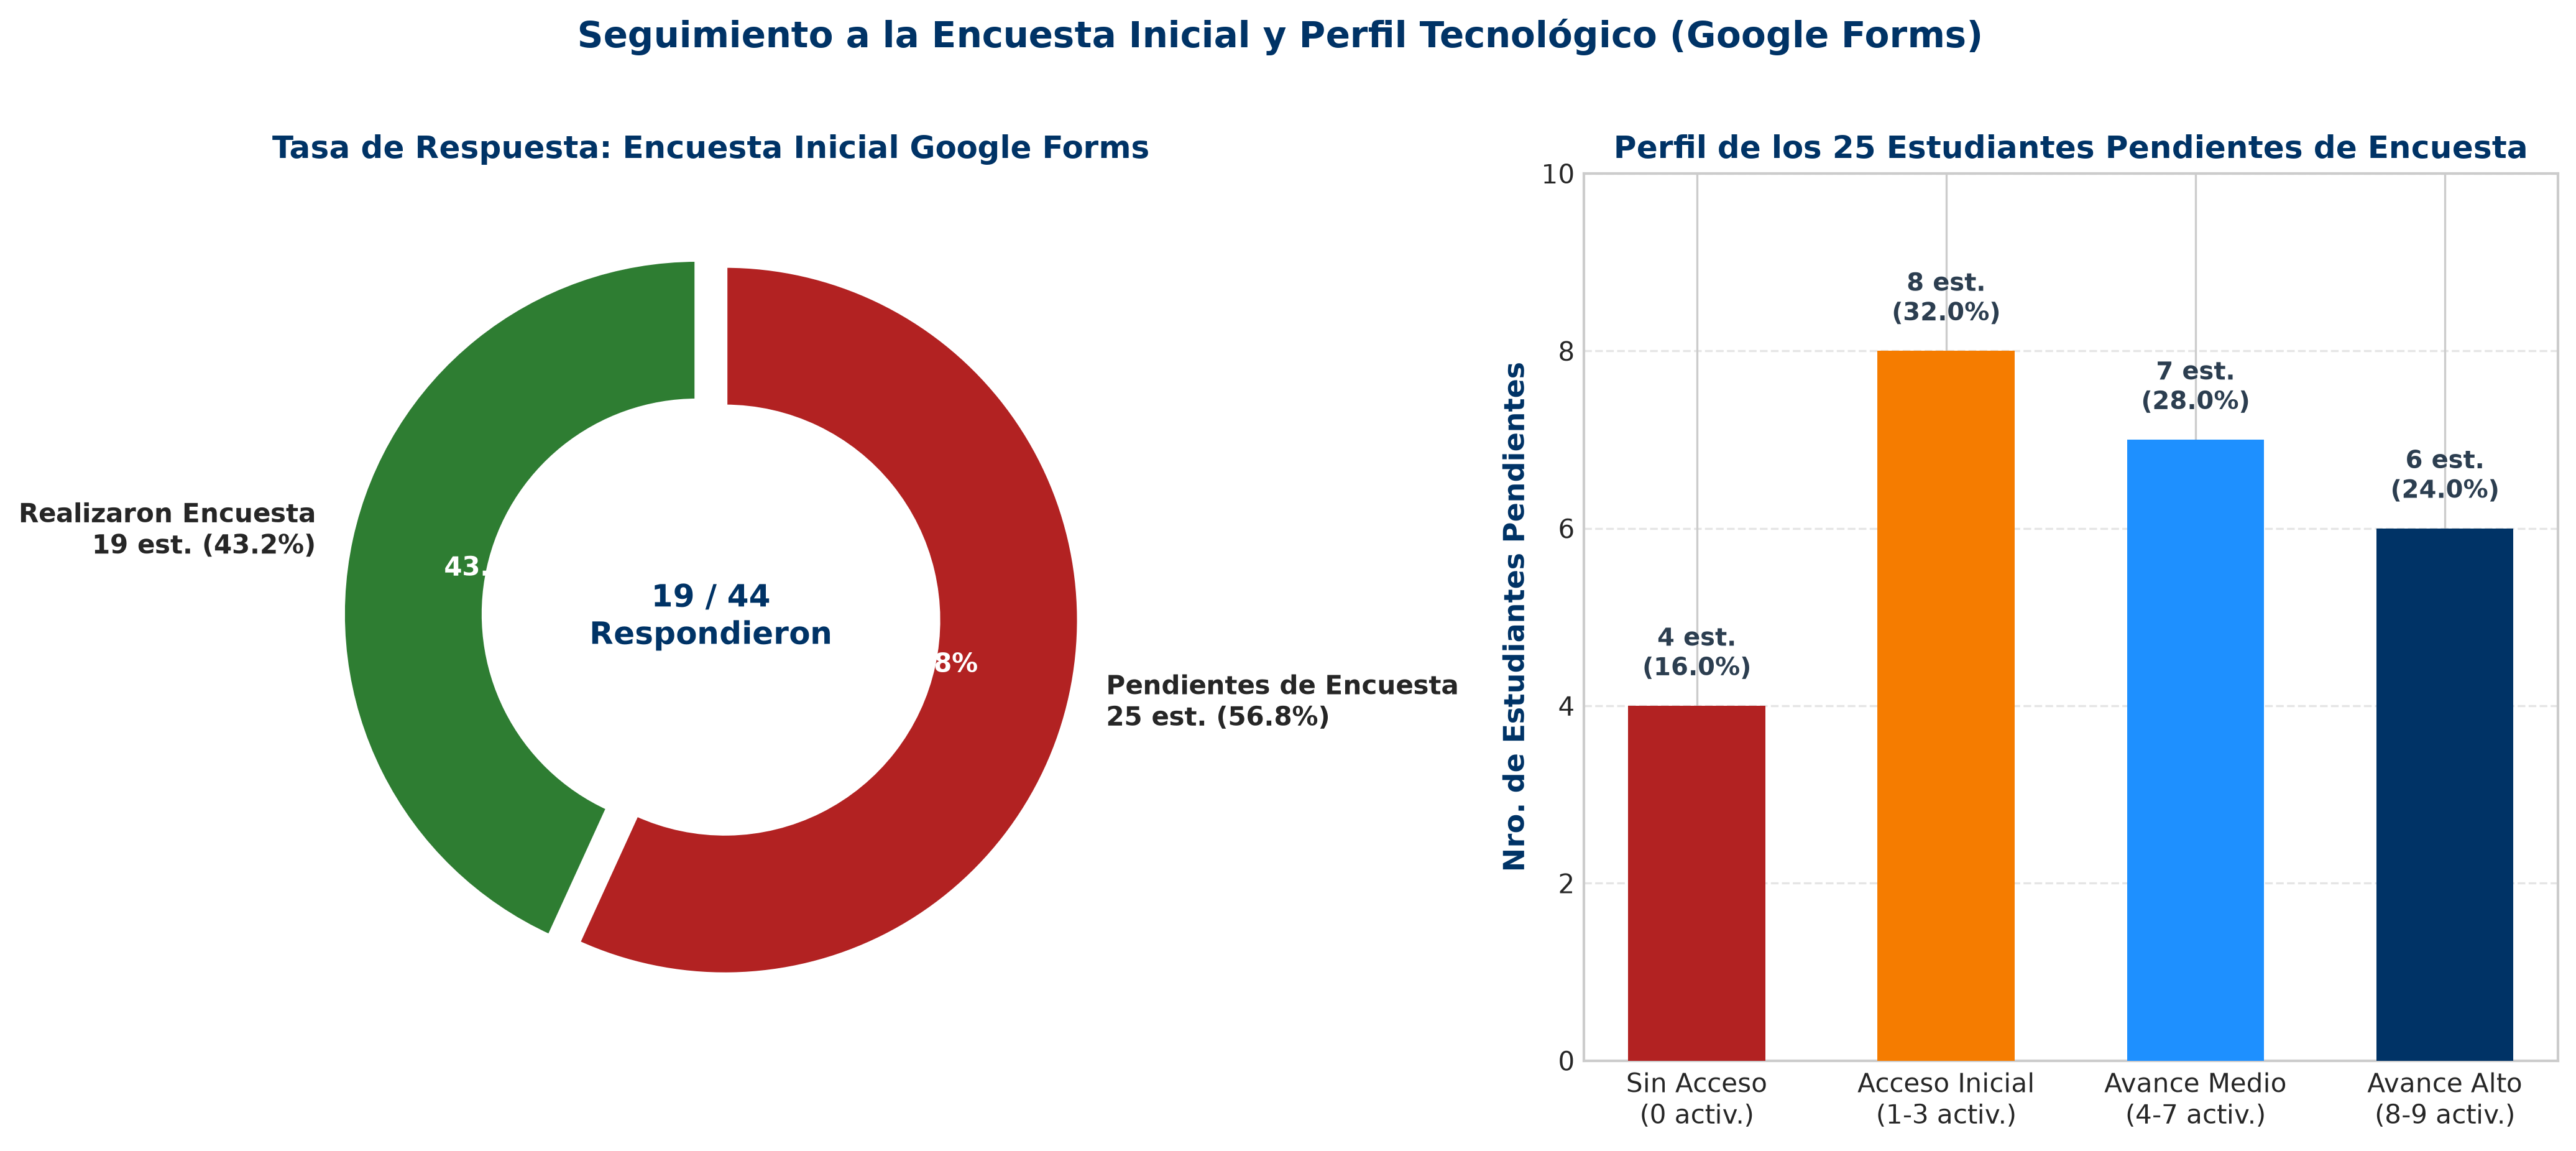
\includegraphics[width=\linewidth]{02_grafico_encuesta_google_torta_barras.png}
    \end{column}
    \begin{column}{0.44\textwidth}
      \begin{block}{Balance de Respuestas}
        \fontsize{7.5}{9.5}\selectfont
        \begin{itemize}
          \item \textbf{Completados:} 19 est. ($43.2\%$).
          \item \textbf{Pendientes:} 25 est. ($56.8\%$).
        \end{itemize}
      \end{block}
      \greenbox{
        \fontsize{7.5}{9.5}\selectfont
        \textbf{Hallazgo Operativo:}\\
        De los 25 pendientes, \textbf{6 estudiantes} (Apaza, Arisaca, Estrada, Quiroz, Urgel, Yucra) ya tienen \textbf{Avance Alto (8/10)} y solo les falta llenar este formulario.
      }
    \end{column}
  \end{columns}
\end{frame}

\begin{frame}{1.6 Comparativa de Hitos Clave del Inicio de Semestre}
  \centering
  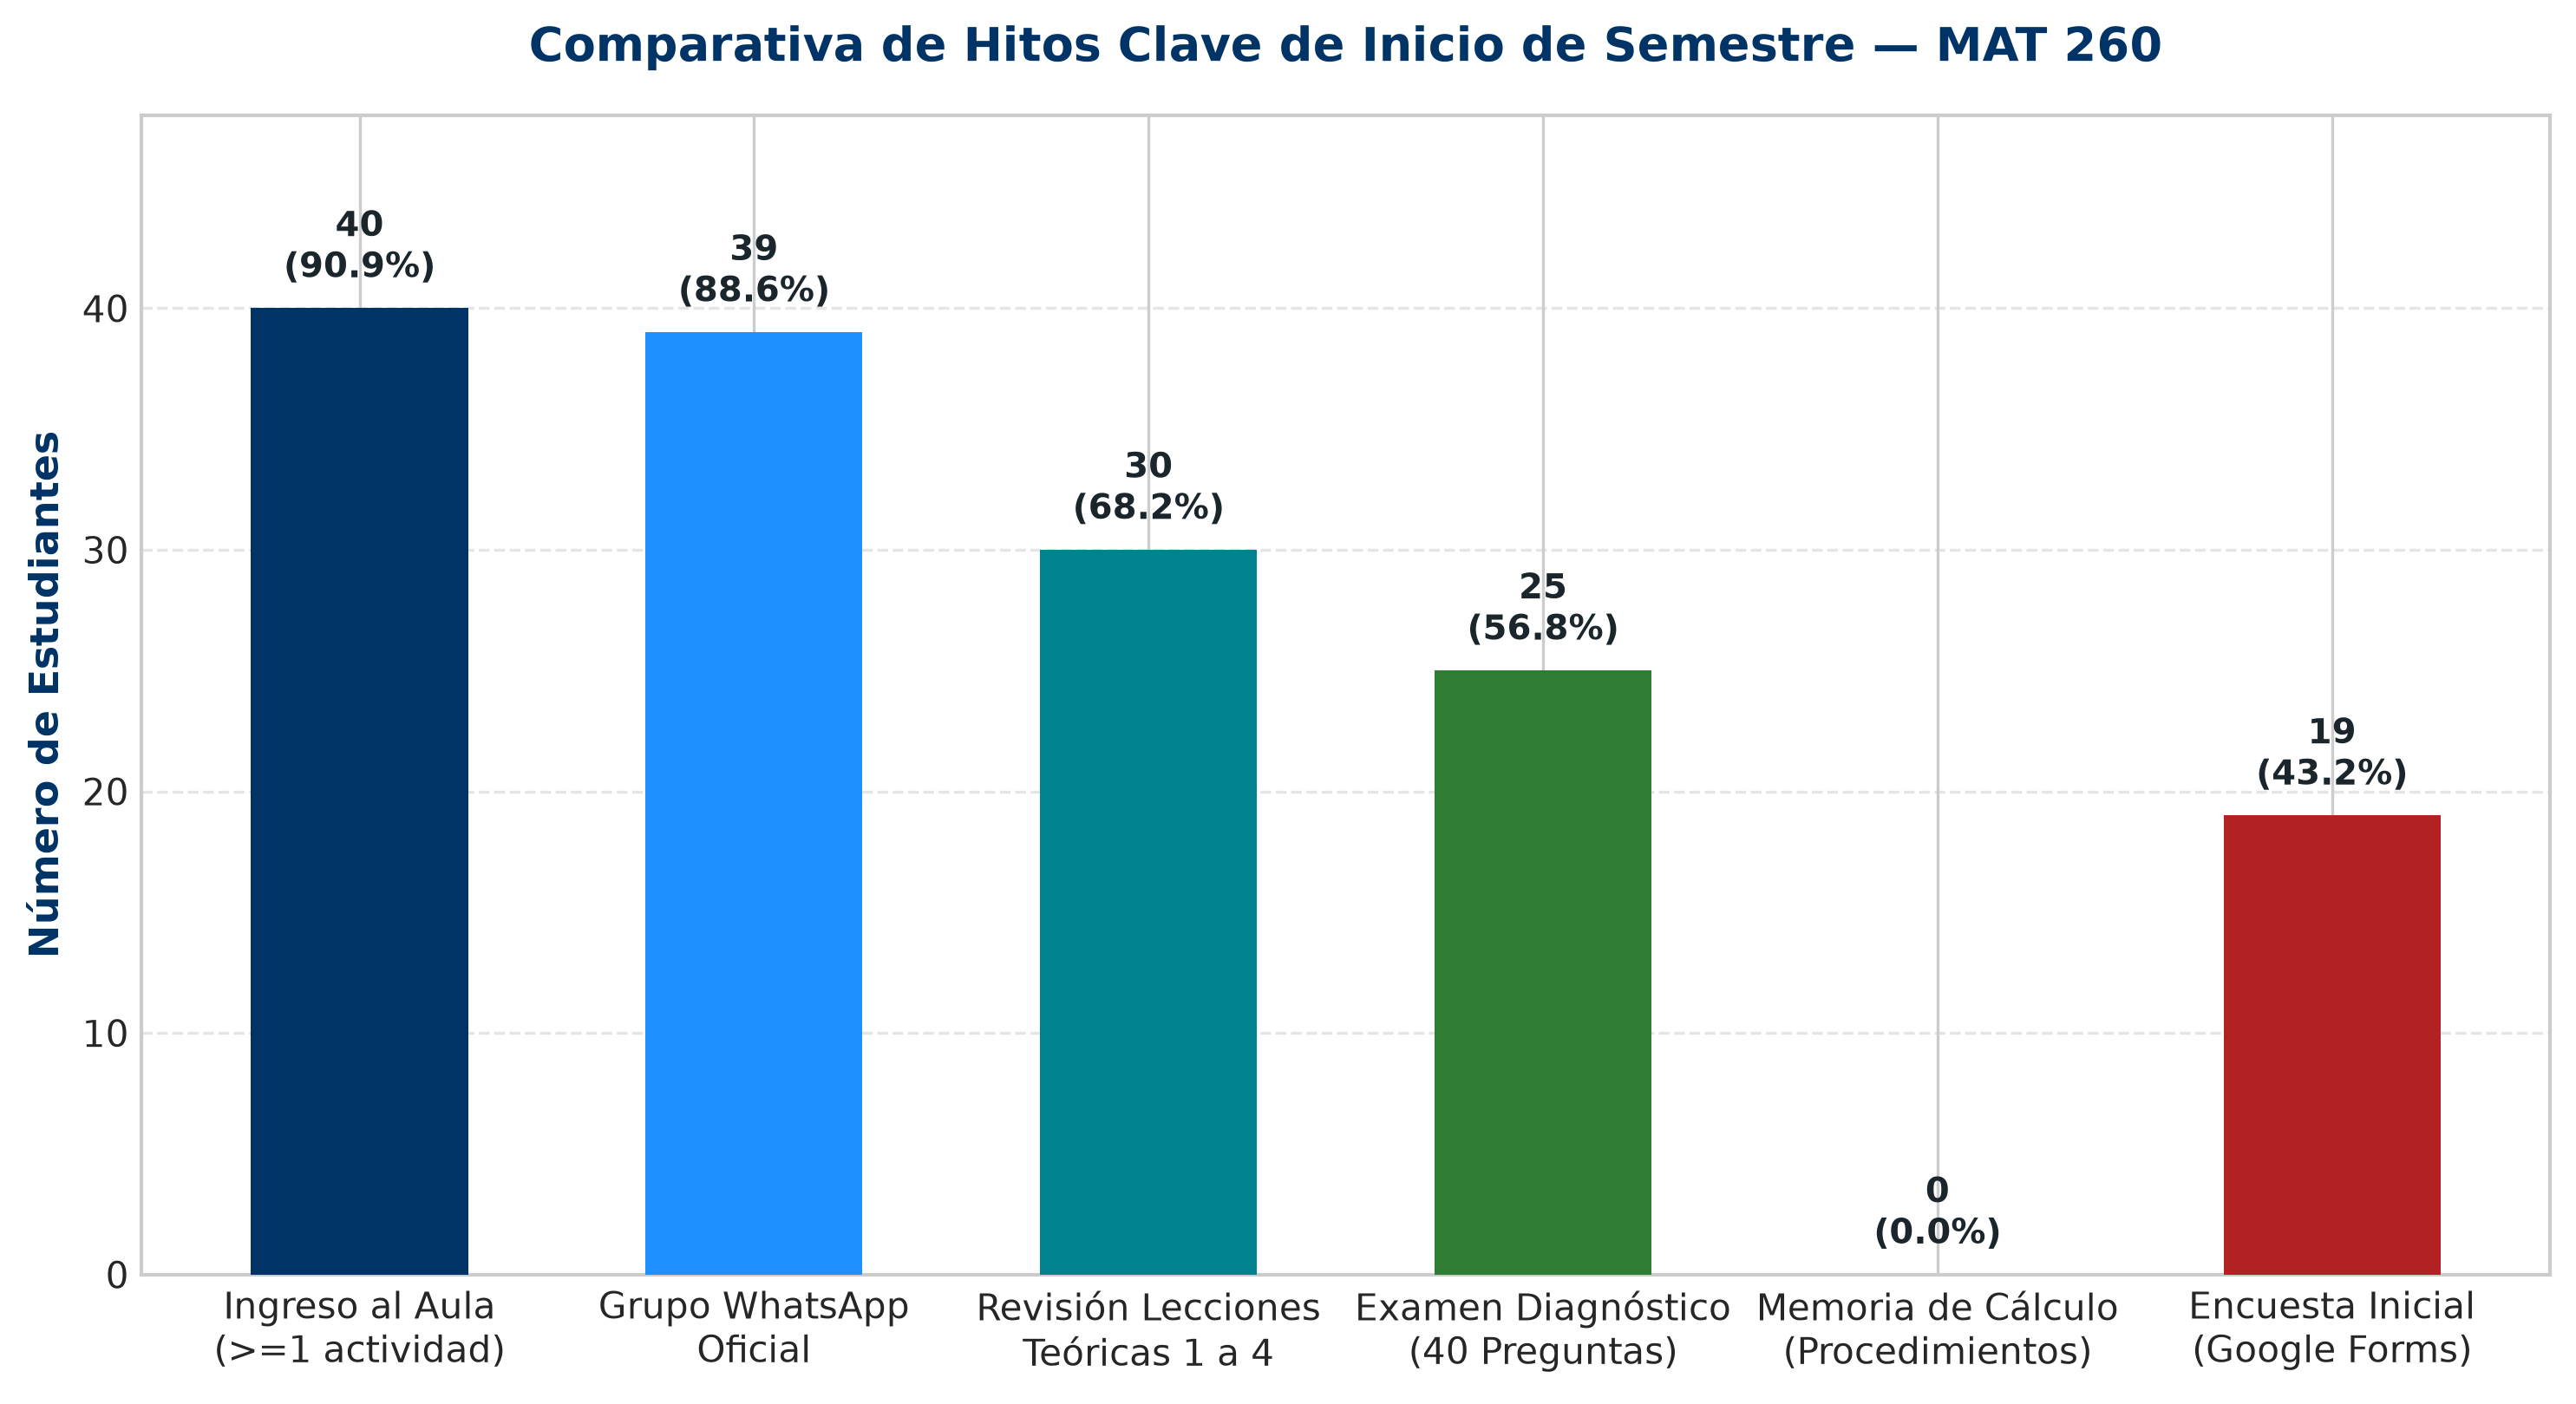
\includegraphics[width=0.88\linewidth]{04_grafico_hitos_clave_barras.png}
\end{frame}

% =========================================================================
% SECCIÓN 2: ANÁLISIS ESTADÍSTICO DE LA ENCUESTA
% =========================================================================
\section{Módulo II: Análisis Estadístico Multivariante de la Encuesta ($N=18$)}

\begin{frame}{2.1 Ficha Metodológica de la Encuesta Diagnóstica}
  \begin{columns}[T]
    \begin{column}{0.48\textwidth}
      \begin{block}{Ficha Técnica}
        \fontsize{7.5}{9.5}\selectfont
        \begin{itemize}
          \item \textbf{Población Objetivo:} 44 estudiantes matriculados (MAT 260).
          \item \textbf{Muestra Efectiva ($n$):} 18 respuestas completas en Google Forms.
          \item \textbf{Tasa de Respuesta:} $40.9\%$.
          \item \textbf{Carrera:} $100\%$ Contaduría Pública / Auditoría.
          \item \textbf{Distribución por Sexo:}
            \begin{itemize}
              \item Femenino: 13 ($72.2\%$)
              \item Masculino: 5 ($27.8\%$)
            \end{itemize}
        \end{itemize}
      \end{block}
    \end{column}
    
    \begin{column}{0.50\textwidth}
      \formulabox{
        \textbf{Clasificación de Variables:}\\[0.1cm]
        \fontsize{7.5}{9.5}\selectfont
        \begin{enumerate}
          \item \textbf{Cuantitativas Continuas:} PPA ($\in [0, 100]$).
          \item \textbf{Cuantitativas Discretas:} Edad en años cumplidos ($X$).
          \item \textbf{Cualitativas Ordinales:} Nivel Excel, Escala Likert de Satisfacción.
          \item \textbf{Cualitativas Nominales:} Sexo, Dispositivo Principal, Modalidad Prácticos.
        \end{enumerate}
      }
    \end{column}
  \end{columns}
\end{frame}

\begin{frame}{2.2 Medidas Descriptivas: Variable Edad}
  \begin{columns}[c]
    \begin{column}{0.48\textwidth}
      \begin{block}{Parámetros de la Edad ($n=18$)}
        \fontsize{7.5}{9.5}\selectfont
        \begin{tabular}{lc}
          \toprule
          \textbf{Estadígrafo} & \textbf{Valor} \\
          \midrule
          Media Aritmética ($\bar{x}$) & \textbf{21.17 años} \\
          Mediana ($Me$) & \textbf{20.00 años} \\
          Moda ($Mo$) & \textbf{19.00 años} \\
          Desviación Estándar ($s$) & \textbf{2.94 años} \\
          Varianza Muestral ($s^2$) & 8.62 años$^2$ \\
          Coeficiente Variación ($CV$) & \textbf{13.9\%} \\
          Rango ($Max - Min$) & 19 a 28 años \\
          Rango Intercuartil ($IQR$) & 3.50 años \\
          Asimetría de Fisher ($g_1$) & \textbf{+1.28 (Positiva)} \\
          Curtosis de Fisher ($g_2$) & +0.37 \\
          \bottomrule
        \end{tabular}
      \end{block}
    \end{column}
    
    \begin{column}{0.50\textwidth}
      \formulabox{
        \textbf{Interpretación Estadística:}\\[0.1cm]
        \fontsize{7.5}{9.5}\selectfont
        $\bar{x} > Me > Mo \implies 21.17 > 20.0 > 19.0$\\[0.1cm]
        Existe un marcado \textbf{sesgo hacia la derecha} ($g_1 = +1.28$). La masa de estudiantes se ubica entre 19 y 20 años, con casos particulares de mayor edad en la cola derecha.
      }
      \vspace{0.1cm}
      \greenbox{
        \fontsize{7.5}{9.5}\selectfont
        \textbf{Baja Dispersión:} $CV = 13.9\% < 20\%$, grupo etario altamente homogéneo.
      }
    \end{column}
  \end{columns}
\end{frame}

\begin{frame}{2.3 Medidas Descriptivas: Promedio Ponderado Acumulado (PPA)}
  \begin{columns}[c]
    \begin{column}{0.48\textwidth}
      \begin{block}{Parámetros del PPA ($n=18$)}
        \fontsize{7.5}{9.5}\selectfont
        \begin{tabular}{lc}
          \toprule
          \textbf{Estadígrafo} & \textbf{Valor} \\
          \midrule
          Media Aritmética ($\bar{y}$) & \textbf{80.81 puntos} \\
          Mediana ($Me$) & \textbf{80.50 puntos} \\
          Moda ($Mo$) & \textbf{92.00 puntos} \\
          Desviación Estándar ($s$) & \textbf{11.24 puntos} \\
          Primer Cuartil ($Q_1$) & 74.50 puntos \\
          Tercer Cuartil ($Q_3$) & 90.75 puntos \\
          Rango ($Max - Min$) & 50.0 a 94.0 pts \\
          Rango Intercuartil ($IQR$) & 16.25 puntos \\
          Asimetría de Fisher ($g_1$) & \textbf{-1.10 (Negativa)} \\
          Curtosis de Fisher ($g_2$) & \textbf{+1.83 (Leptocúrtica)} \\
          \bottomrule
        \end{tabular}
      \end{block}
    \end{column}
    
    \begin{column}{0.50\textwidth}
      \greenbox{
        \textbf{Perfil de Excelencia Académica:}\\[0.1cm]
        \fontsize{7.5}{9.5}\selectfont
        $\blacktriangleright$ El \textbf{75\% del curso} tiene un PPA $\ge 74.5$ puntos.\\
        $\blacktriangleright$ La asimetría negativa ($g_1 = -1.10$) indica concentración en calificaciones de alto rendimiento (80 a 94 pts).\\
        $\blacktriangleright$ La moda en 92.0 pts denota un grupo con sólidos antecedentes formativos.
      }
    \end{column}
  \end{columns}
\end{frame}

\begin{frame}{2.4 Perfil Demográfico y Académico Integrado}
  \centering
  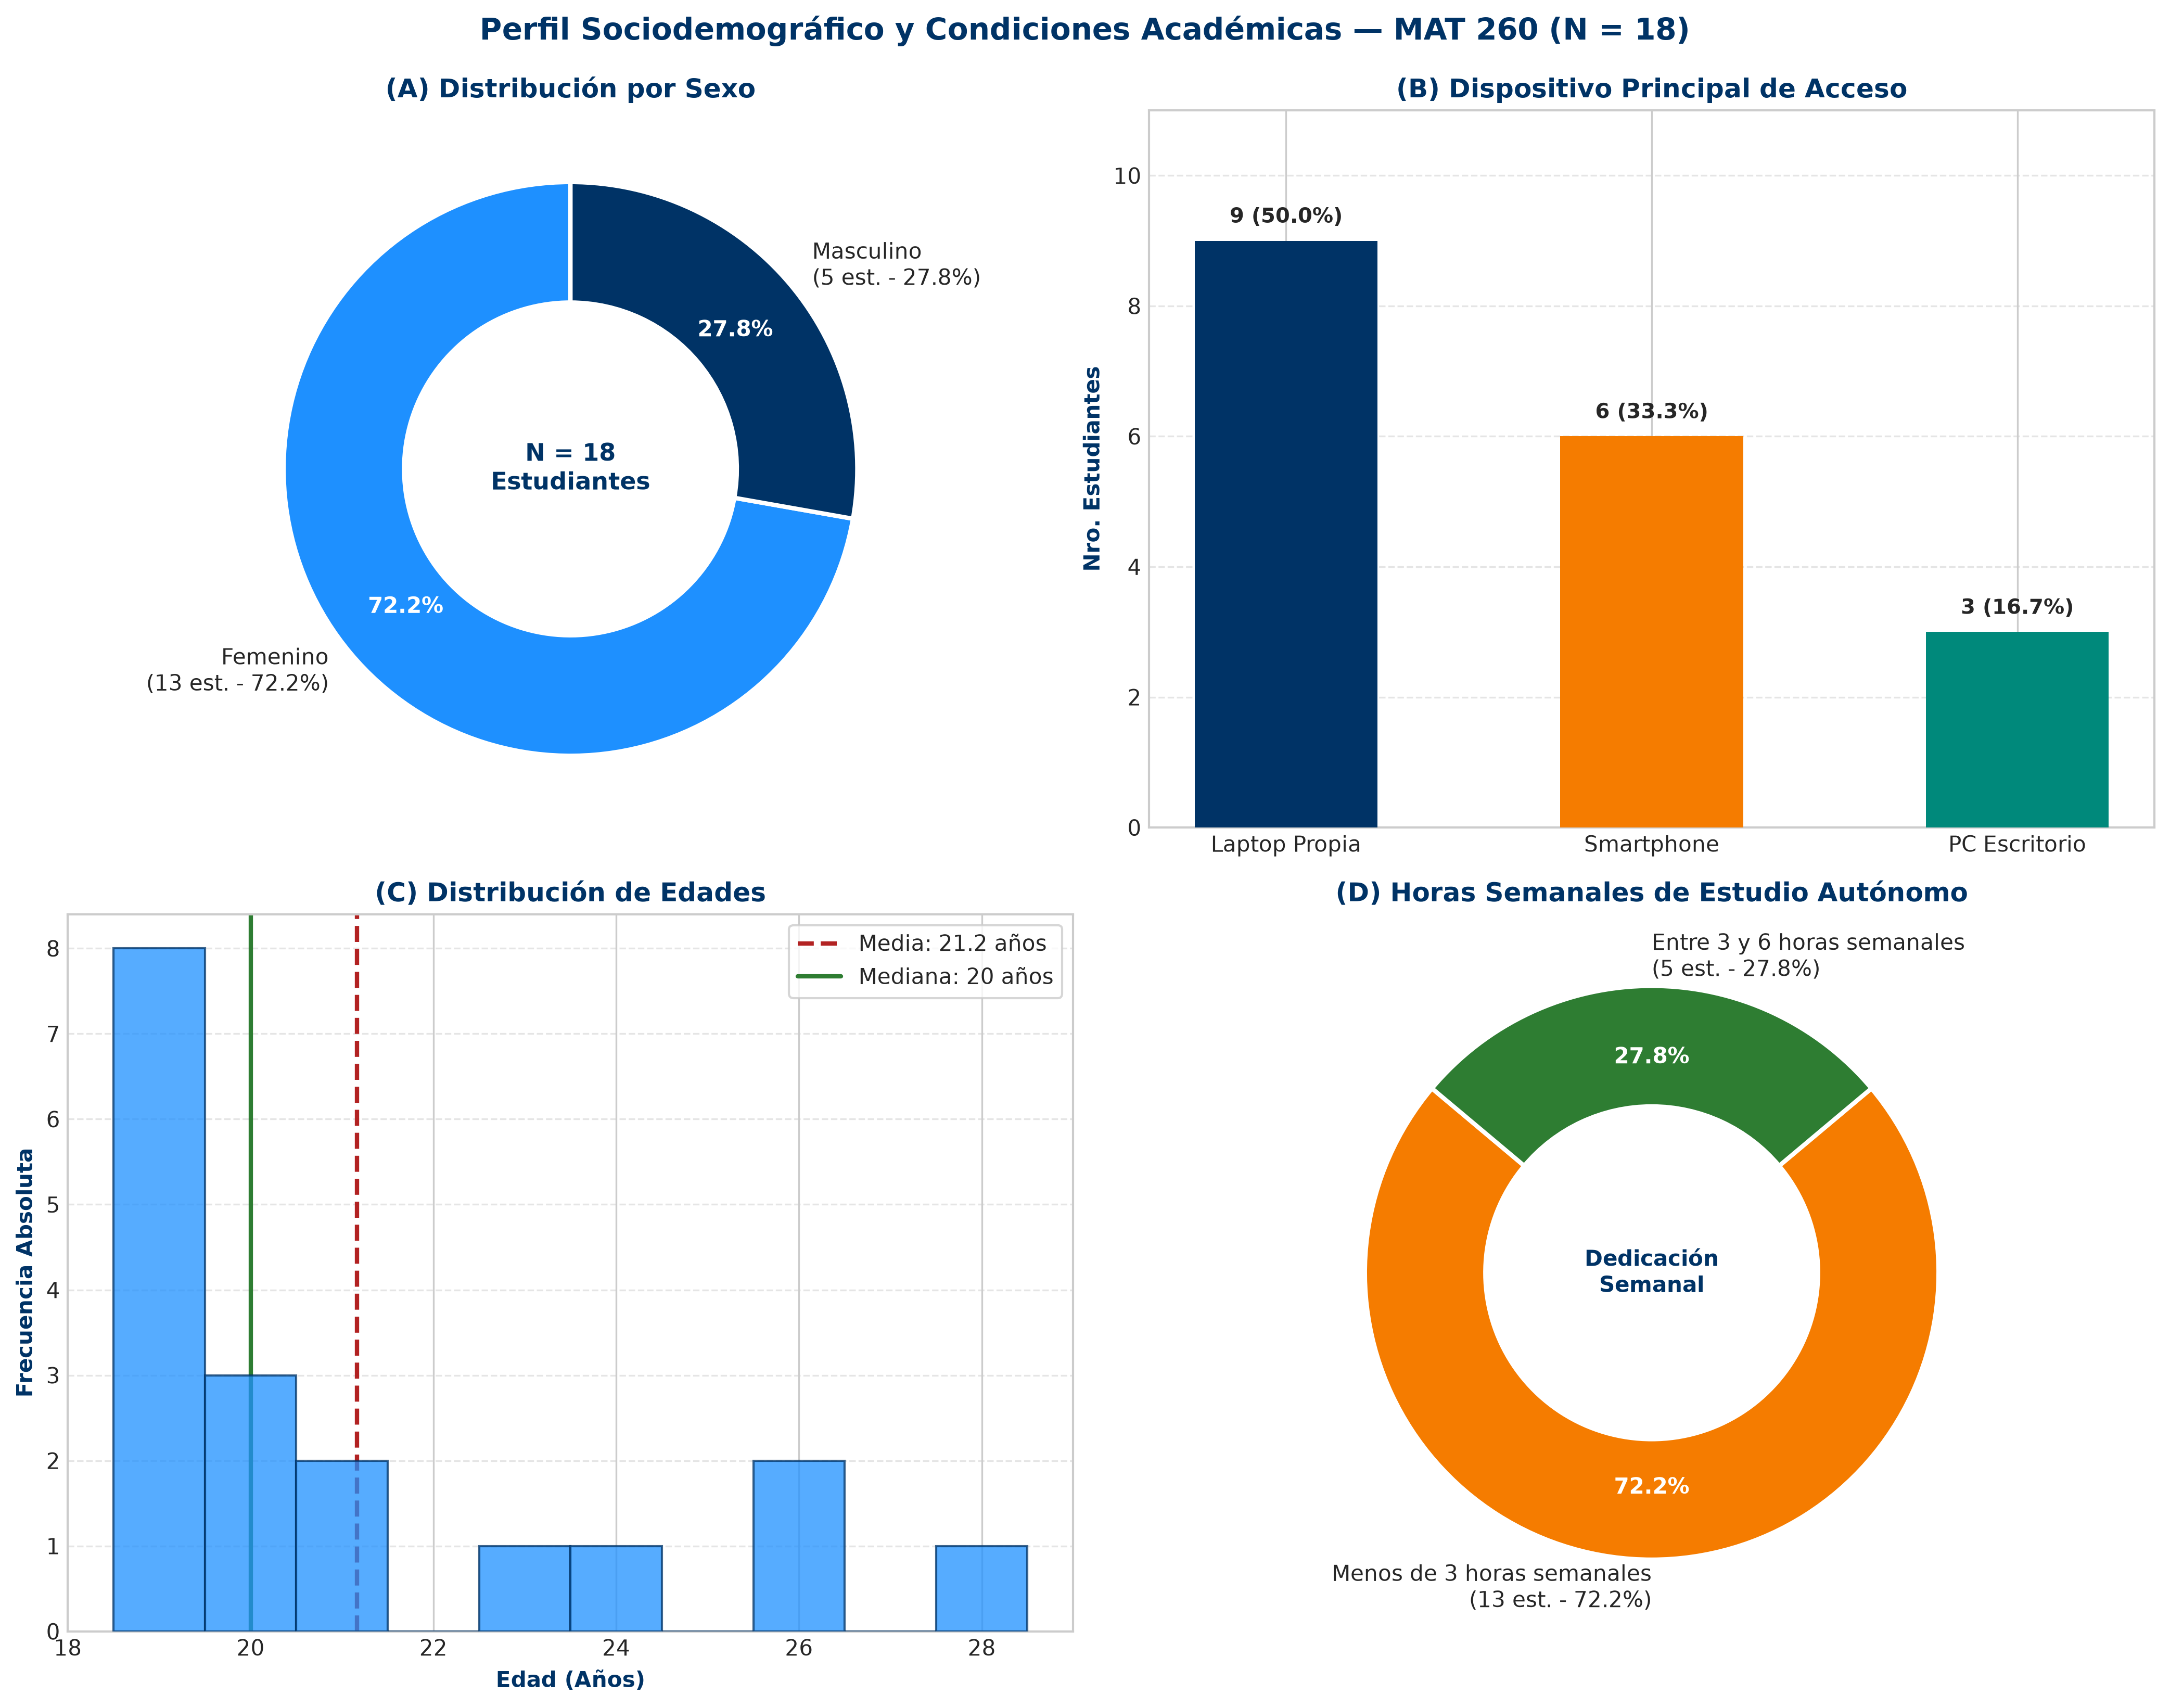
\includegraphics[width=0.88\linewidth]{01_perfil_demografico_academico.png}
\end{frame}

\begin{frame}{2.5 Perfil Tecnológico y Competencias Digitales}
  \centering
  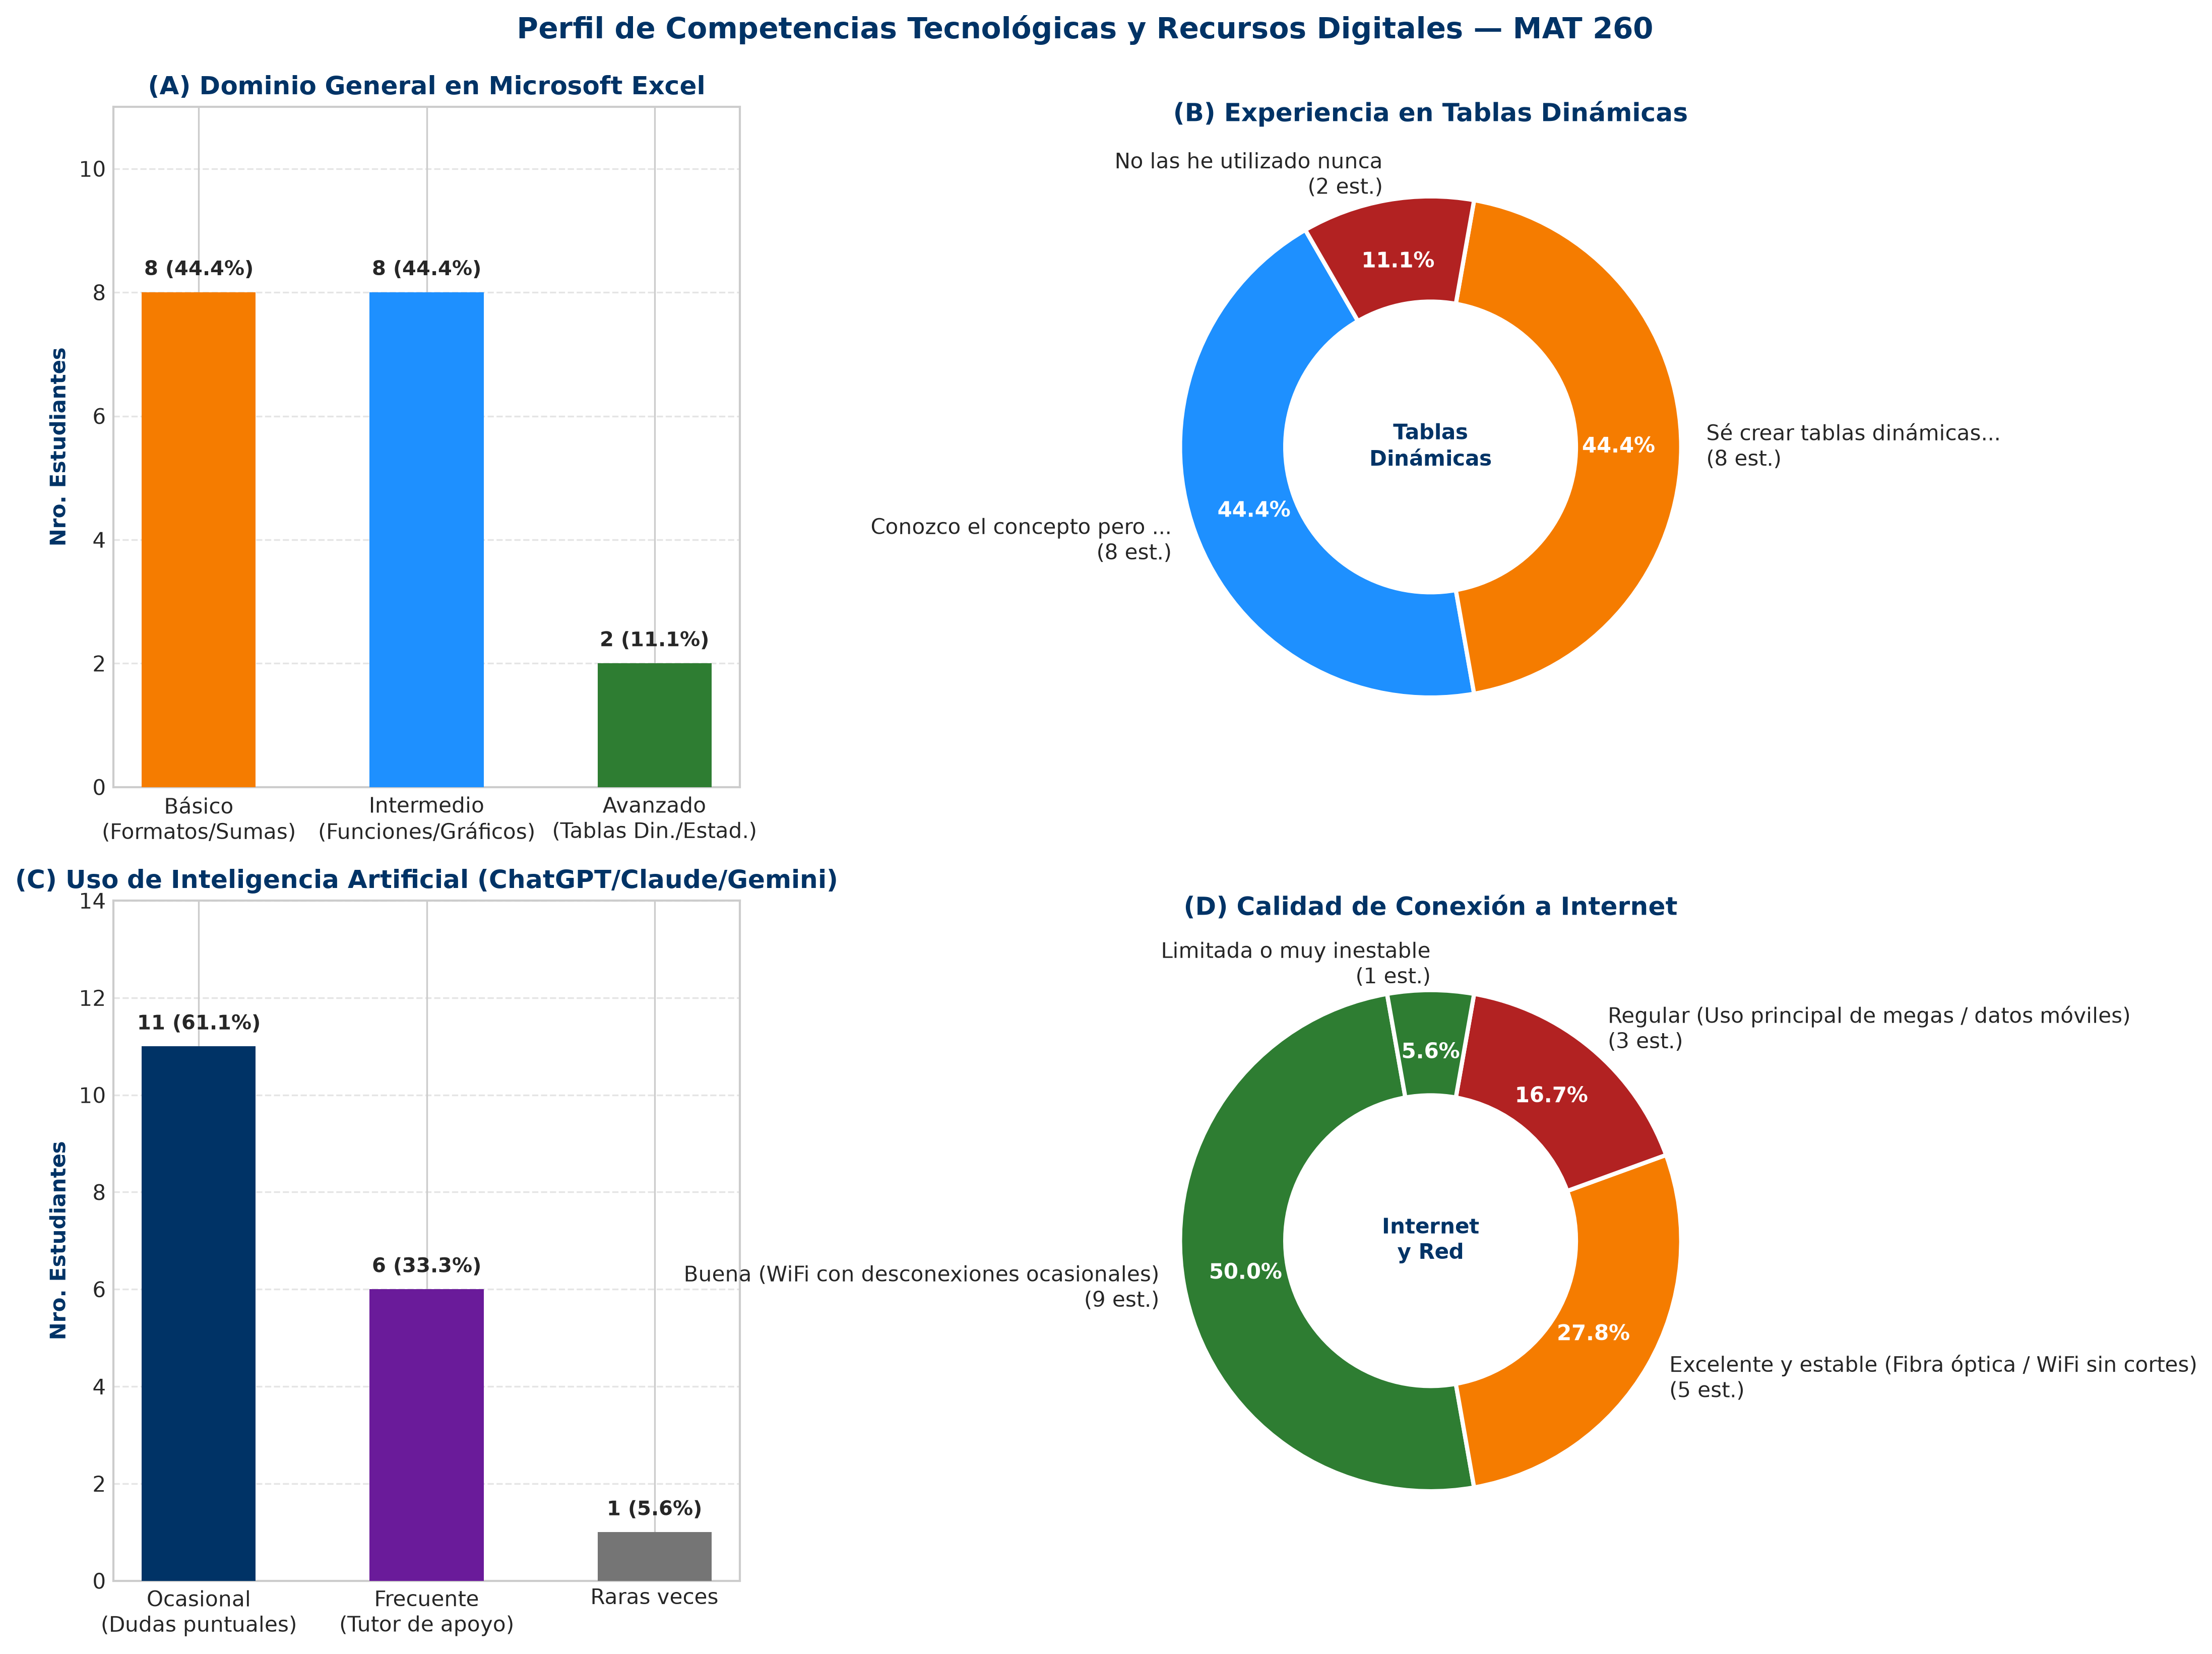
\includegraphics[width=0.88\linewidth]{02_perfil_tecnologico_excel_ia.png}
  
  \vspace{0.05cm}
  \fontsize{7.5}{9.5}\selectfont
  \textbf{Hallazgos Clave:} $88.9\%$ está en nivel básico/intermedio en Excel. \textbf{94.4\% ya utiliza IA} para estudiar.
\end{frame}

\begin{frame}{2.6 Evaluación Pedagógica de la Activación y Examen Diagnóstico}
  \centering
  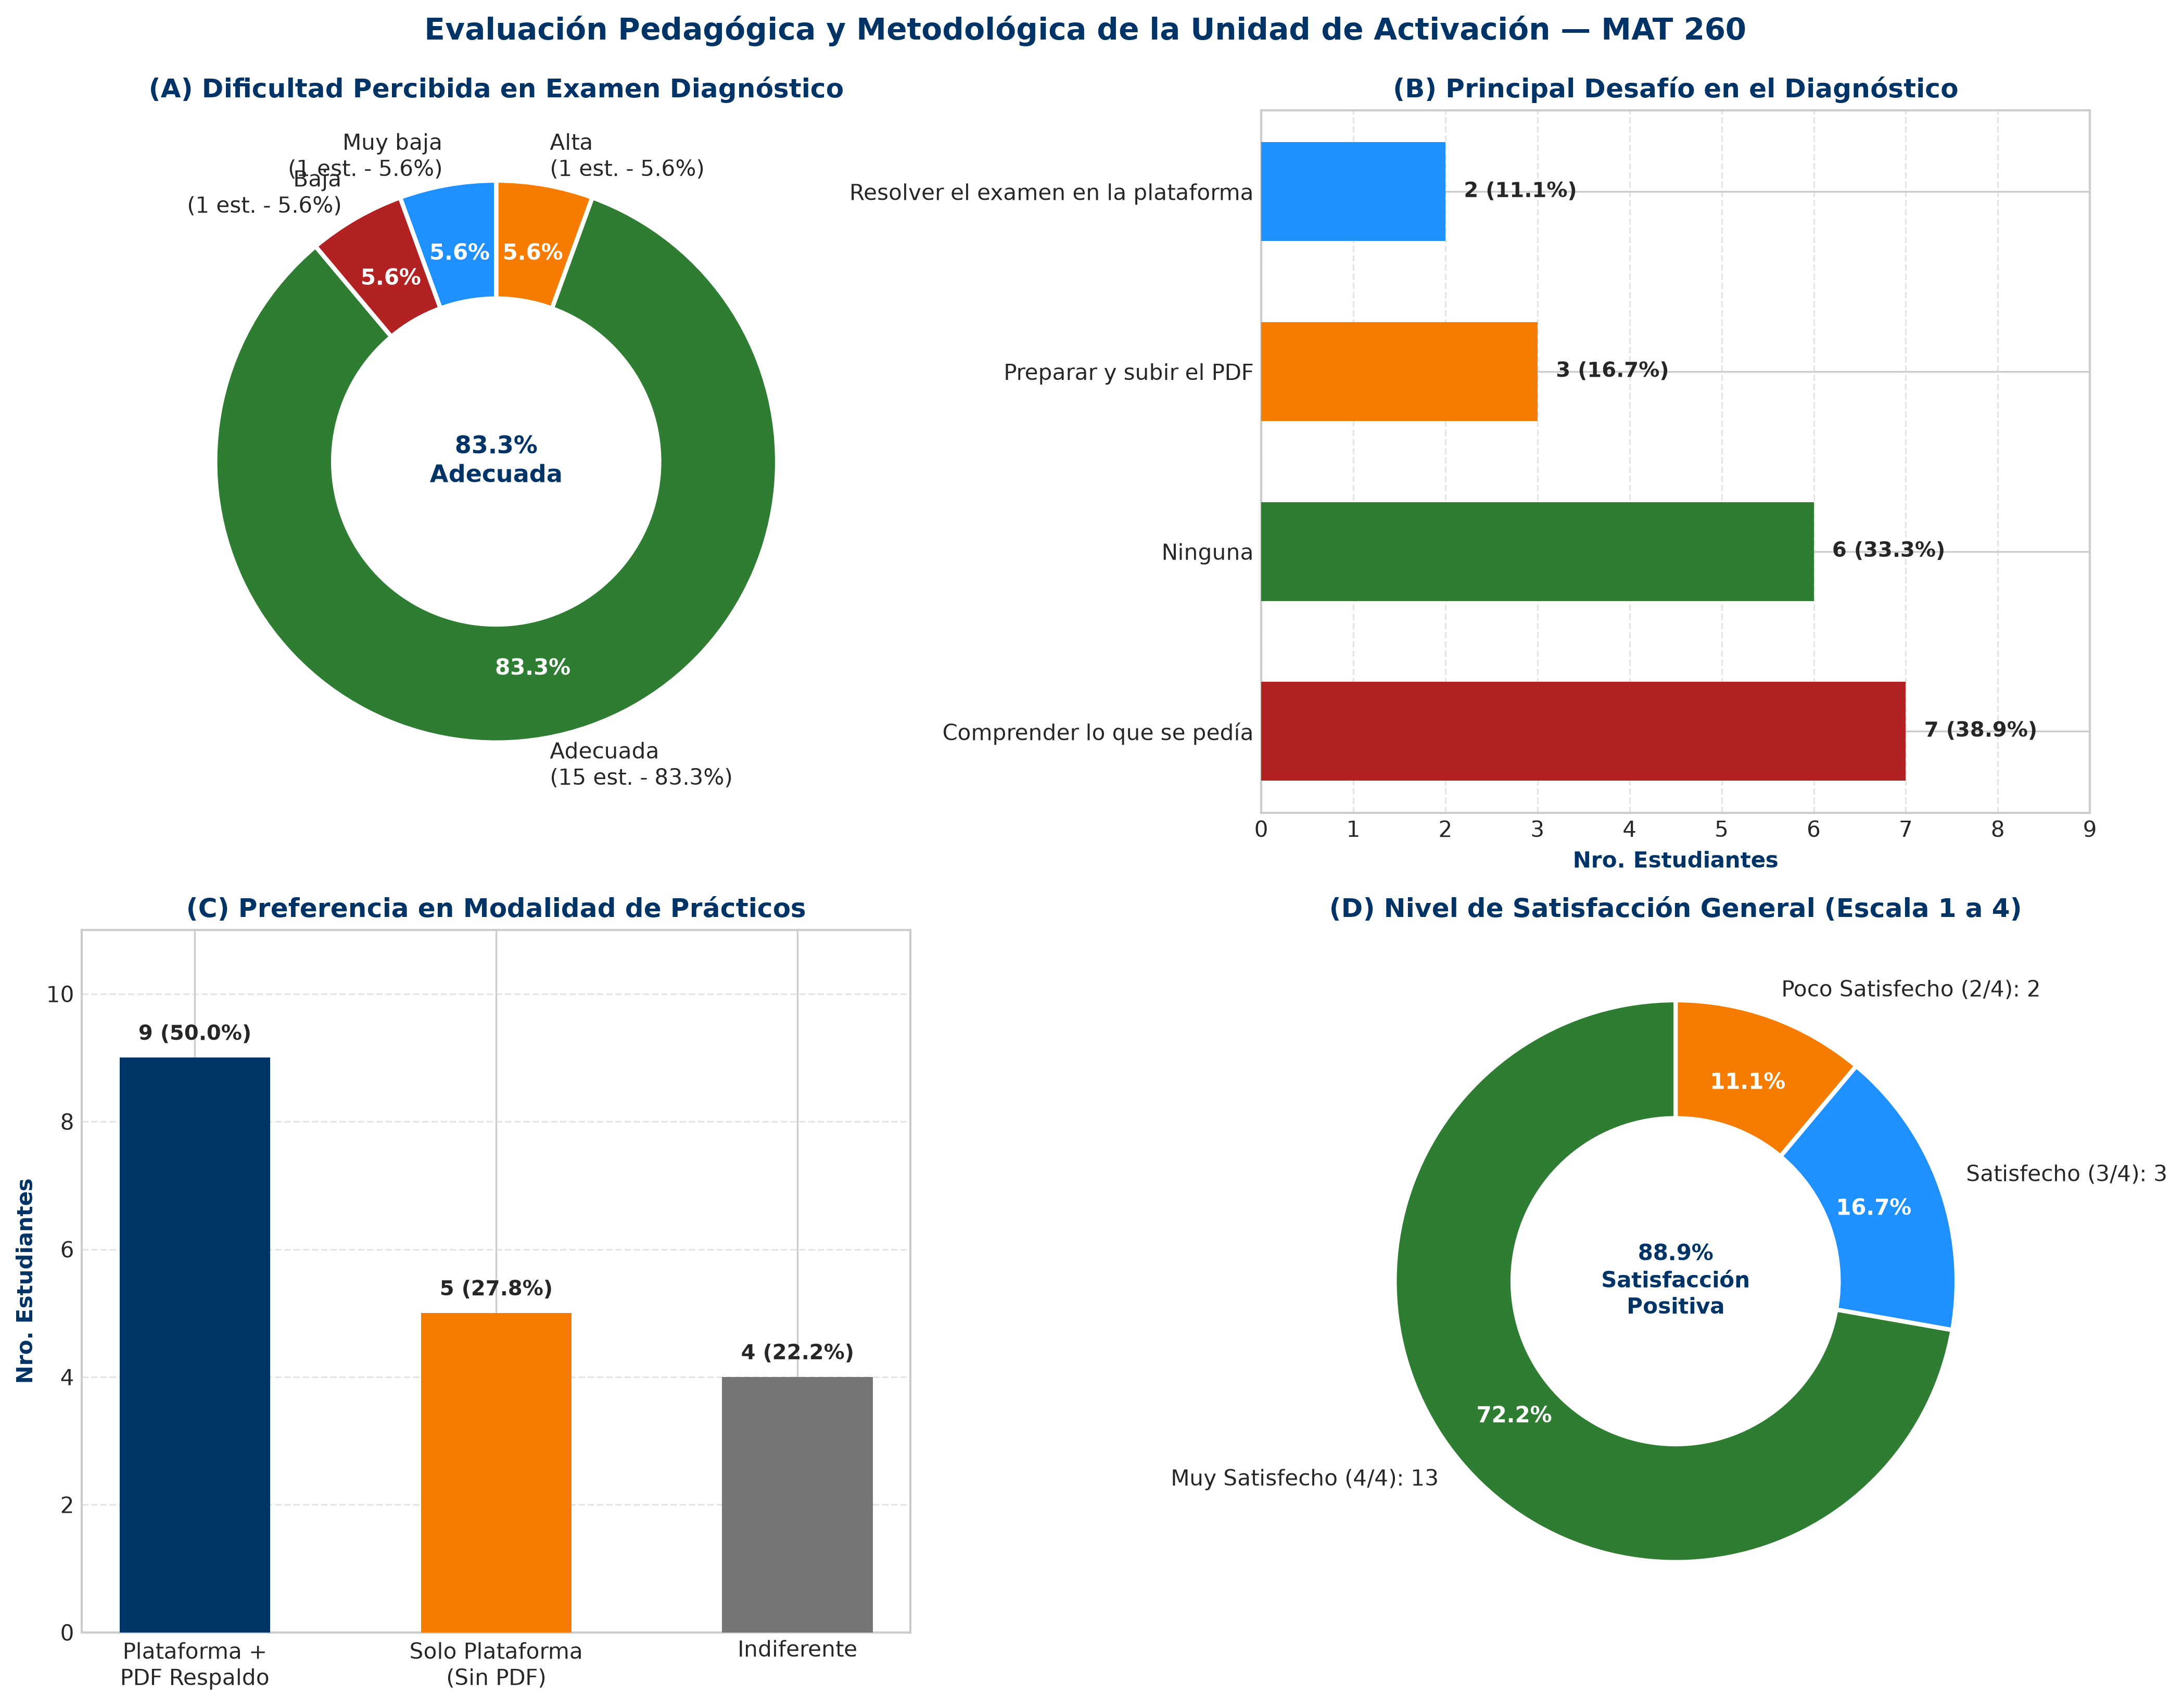
\includegraphics[width=0.88\linewidth]{03_evaluacion_pedagogica_satisfaccion.png}
\end{frame}

\begin{frame}{2.7 Análisis Bivariado y Tablas de Contingencia}
  \begin{columns}[T]
    \begin{column}{0.48\textwidth}
      \begin{block}{Sexo vs. Dominio en Excel}
        \fontsize{7}{9}\selectfont
        \begin{tabular}{lcccc}
          \toprule
          \textbf{Sexo} & \textbf{Básico} & \textbf{Interm.} & \textbf{Avanz.} & \textbf{Total} \\
          \midrule
          Femenino & 6 & 5 & 2 & 13 \\
          Masculino & 2 & 3 & 0 & 5 \\
          \midrule
          \textbf{Total} & \textbf{8} & \textbf{8} & \textbf{2} & \textbf{18} \\
          \bottomrule
        \end{tabular}
      \end{block}
      
      \begin{block}{Dispositivo vs. Modalidad Prácticos}
        \fontsize{7}{9}\selectfont
        \begin{tabular}{lcccc}
          \toprule
          \textbf{Dispositivo} & \textbf{PDF} & \textbf{Sin PDF} & \textbf{Indif.} & \textbf{Total} \\
          \midrule
          Laptop & 5 & 2 & 2 & 9 \\
          Smartphone & 2 & \alert{\textbf{3}} & 1 & 6 \\
          PC Escritorio & 2 & 0 & 1 & 3 \\
          \midrule
          \textbf{Total} & \textbf{9} & \textbf{5} & \textbf{4} & \textbf{18} \\
          \bottomrule
        \end{tabular}
      \end{block}
    \end{column}
    
    \begin{column}{0.50\textwidth}
      \centering
      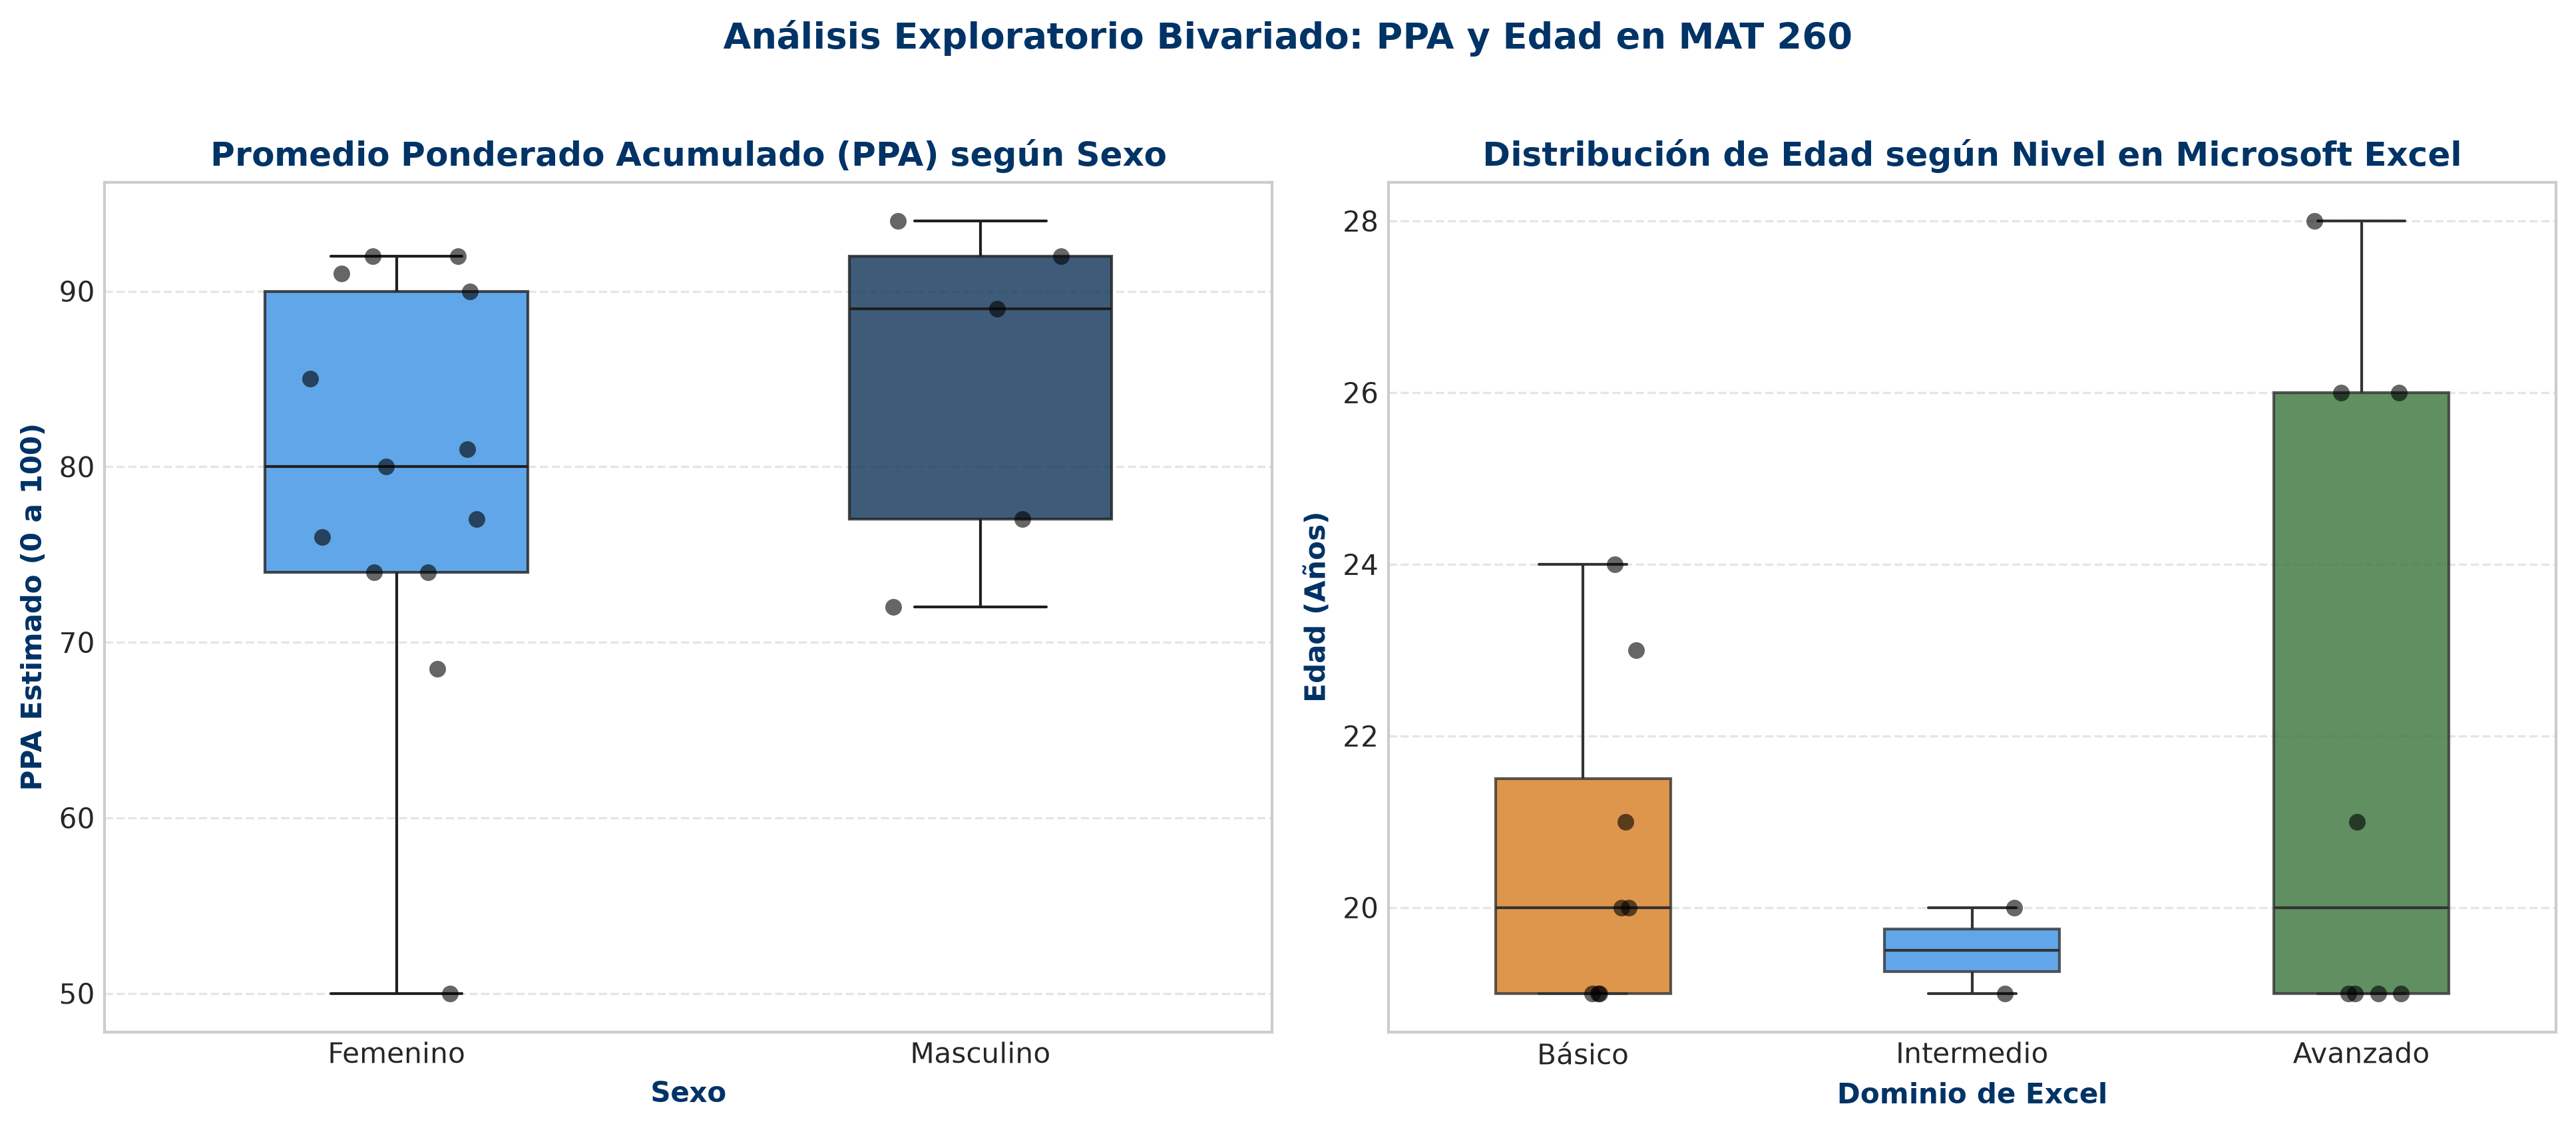
\includegraphics[width=\linewidth]{04_analisis_bivariado_ppa_edad.png}
      \vspace{0.05cm}
      \formulabox{
        \fontsize{7}{9}\selectfont
        \textbf{Correlación de Factores:} Los usuarios de Smartphone muestran mayor inclinación a entregas directas sin PDF por dificultad de digitalización móvil.
      }
    \end{column}
  \end{columns}
\end{frame}

\begin{frame}{2.8 Análisis Cualitativo: Expectativas de los Estudiantes}
  \begin{block}{Síntesis Temática de Comentarios Abiertos}
    \fontsize{7.5}{9.5}\selectfont
    \begin{enumerate}
      \item \textbf{Puente con Estadística I (50\% menciones):} Deseo expreso de afianzar conceptos previos para no confundir medidas descriptivas con modelos estocásticos.
      \item \textbf{Aplicación Práctica Contable (35\% menciones):} Interés en resolver casos de auditoría, riesgos y toma de decisiones gerenciales.
      \item \textbf{Talleres en Computadora (25\% menciones):} Aprender a trasladar el cálculo manual a hojas estructuradas de Excel.
      \item \textbf{Claridad en Enunciados:} Énfasis en resolver variedad de problemas tipo examen.
    \end{enumerate}
  \end{block}
  
  \formulabox{
    \fontsize{7.5}{9.5}\selectfont
    \textit{“Mis expectativas para Estadística II son comprender mejor los temas, desarrollar la capacidad de interpretar datos y aprender a comunicar los hallazgos para la toma de decisiones.”} — Estudiante MAT 260
  }
\end{frame}

% =========================================================================
% SECCIÓN 3: PAUTAS PEDAGÓGICAS Y PLAN DE ACCIÓN
% =========================================================================
\section{Módulo III: Pautas Pedagógicas y Plan de Acción Docente}

\begin{frame}{3.1 Reflexiones para Compartir en Clase Presencial}
  \greenbox{
    \textbf{Mensajes Clave para Motivar al Estudiante:}\\[0.1cm]
    \fontsize{7.5}{9.5}\selectfont
    \begin{itemize}
      \item \textbf{1. Confianza en su Capacidad:} Presentarles su PPA promedio de \textbf{80.8 puntos} para reafirmar que tienen un perfil de alto desempeño.
      \item \textbf{2. La Estadística como Herramienta Decisional:} Demostrarles con este mismo informe cómo los datos de su curso permiten planificar estrategias pedagógicas reales.
      \item \textbf{3. Inteligencia Artificial como Copiloto:} El $94.4\%$ ya la usa; se les enseñará a formular prompts analíticos para validación y profundización.
      \item \textbf{4. Nivelación Progresiva en Excel:} Nadie se quedará atrás; las fórmulas y tablas se construirán paso a paso en clases y laboratorios.
    \end{itemize}
  }
\end{frame}

\begin{frame}{3.2 Plan de Acción Docente Inmediato}
  \begin{columns}[T]
    \begin{column}{0.48\textwidth}
      \begin{block}{Línea de Acción Inmediata}
        \fontsize{7.5}{9.5}\selectfont
        \begin{itemize}
          \item \textbf{Contacto de Rescate:} Llamar a Esmeralda Vejar y notificar a los 3 casos sin acceso en el aula física.
          \item \textbf{Cierre de Encuesta Google:} Recordatorio directo a los 6 estudiantes con avance 8/10 para alcanzar $100\%$ de respuestas.
          \item \textbf{Inicio Unidad 1:} Arrancar con Análisis Combinatorio articulando teoría manual y verificación algorítmica.
        \end{itemize}
      \end{block}
    \end{column}
    
    \begin{column}{0.50\textwidth}
      \formulabox{
        \textbf{Compromiso Institucional:}\\[0.1cm]
        \fontsize{7.5}{9.5}\selectfont
        Garantizar una experiencia de aprendizaje universitaria de máxima calidad, combinando rigor matemático, aplicaciones contables, entornos virtuales dinámicos y formación tecnológica de vanguardia.
      }
    \end{column}
  \end{columns}
\end{frame}

% =========================================================================
% CIERRE
% =========================================================================
\begin{frame}[plain]
  \centering
  \vspace{0.8cm}
  \begin{minipage}{0.30\textwidth}
    \centering
    
\includegraphics[width=0.65\linewidth]{Logouagrm.png}
  \end{minipage}
  \hfill
  \begin{minipage}{0.30\textwidth}
    \centering
    
\includegraphics[width=0.65\linewidth]{Logocont.png}
  \end{minipage}
  
  \vspace{0.5cm}
  {\large \textbf{\color{darkblue}¡MUCHAS GRACIAS POR SU ATENCIÓN!}}\\[0.2cm]
  {\small \textbf{\color{dodgerblue}Estadística II (MAT 260 - Grupo EP)}}\\[0.1cm]
  {\footnotesize Facultad de Ciencias Contables, Auditoría, Sistemas de Control de Gestión y Finanzas}\\[0.1cm]
  {\footnotesize Universidad Autónoma Gabriel René Moreno}\\[0.4cm]
  
  \begin{beamercolorbox}[sep=4pt,center,rounded=true]{palette secondary}
    \footnotesize \textbf{MSc. Ing. Anselmo Salguero Arano} — Docente Titular UAGRM
  \end{beamercolorbox}
\end{frame}

\end{document}
